\documentclass[]{article}
\usepackage{lmodern}
\usepackage{amssymb,amsmath}
\usepackage{ifxetex,ifluatex}
\usepackage{fixltx2e} % provides \textsubscript
\ifnum 0\ifxetex 1\fi\ifluatex 1\fi=0 % if pdftex
  \usepackage[T1]{fontenc}
  \usepackage[utf8]{inputenc}
\else % if luatex or xelatex
  \ifxetex
    \usepackage{mathspec}
  \else
    \usepackage{fontspec}
  \fi
  \defaultfontfeatures{Ligatures=TeX,Scale=MatchLowercase}
\fi
% use upquote if available, for straight quotes in verbatim environments
\IfFileExists{upquote.sty}{\usepackage{upquote}}{}
% use microtype if available
\IfFileExists{microtype.sty}{%
\usepackage{microtype}
\UseMicrotypeSet[protrusion]{basicmath} % disable protrusion for tt fonts
}{}
\usepackage[margin=1in]{geometry}
\usepackage{hyperref}
\hypersetup{unicode=true,
            pdfborder={0 0 0},
            breaklinks=true}
\urlstyle{same}  % don't use monospace font for urls
\usepackage{graphicx,grffile}
\makeatletter
\def\maxwidth{\ifdim\Gin@nat@width>\linewidth\linewidth\else\Gin@nat@width\fi}
\def\maxheight{\ifdim\Gin@nat@height>\textheight\textheight\else\Gin@nat@height\fi}
\makeatother
% Scale images if necessary, so that they will not overflow the page
% margins by default, and it is still possible to overwrite the defaults
% using explicit options in \includegraphics[width, height, ...]{}
\setkeys{Gin}{width=\maxwidth,height=\maxheight,keepaspectratio}
\IfFileExists{parskip.sty}{%
\usepackage{parskip}
}{% else
\setlength{\parindent}{0pt}
\setlength{\parskip}{6pt plus 2pt minus 1pt}
}
\setlength{\emergencystretch}{3em}  % prevent overfull lines
\providecommand{\tightlist}{%
  \setlength{\itemsep}{0pt}\setlength{\parskip}{0pt}}
\setcounter{secnumdepth}{0}
% Redefines (sub)paragraphs to behave more like sections
\ifx\paragraph\undefined\else
\let\oldparagraph\paragraph
\renewcommand{\paragraph}[1]{\oldparagraph{#1}\mbox{}}
\fi
\ifx\subparagraph\undefined\else
\let\oldsubparagraph\subparagraph
\renewcommand{\subparagraph}[1]{\oldsubparagraph{#1}\mbox{}}
\fi

%%% Use protect on footnotes to avoid problems with footnotes in titles
\let\rmarkdownfootnote\footnote%
\def\footnote{\protect\rmarkdownfootnote}

%%% Change title format to be more compact
\usepackage{titling}

% Create subtitle command for use in maketitle
\providecommand{\subtitle}[1]{
  \posttitle{
    \begin{center}\large#1\end{center}
    }
}

\setlength{\droptitle}{-2em}

  \title{}
    \pretitle{\vspace{\droptitle}}
  \posttitle{}
    \author{}
    \preauthor{}\postauthor{}
    \date{}
    \predate{}\postdate{}
  

\begin{document}

\FloatBarrier
\newpage

\hypertarget{figures}{%
\section{Figures}\label{figures}}

\hypertarget{data-figures}{%
\subsection{Data Figures}\label{data-figures}}

\begin{figure}[!h]
\begin{centering}
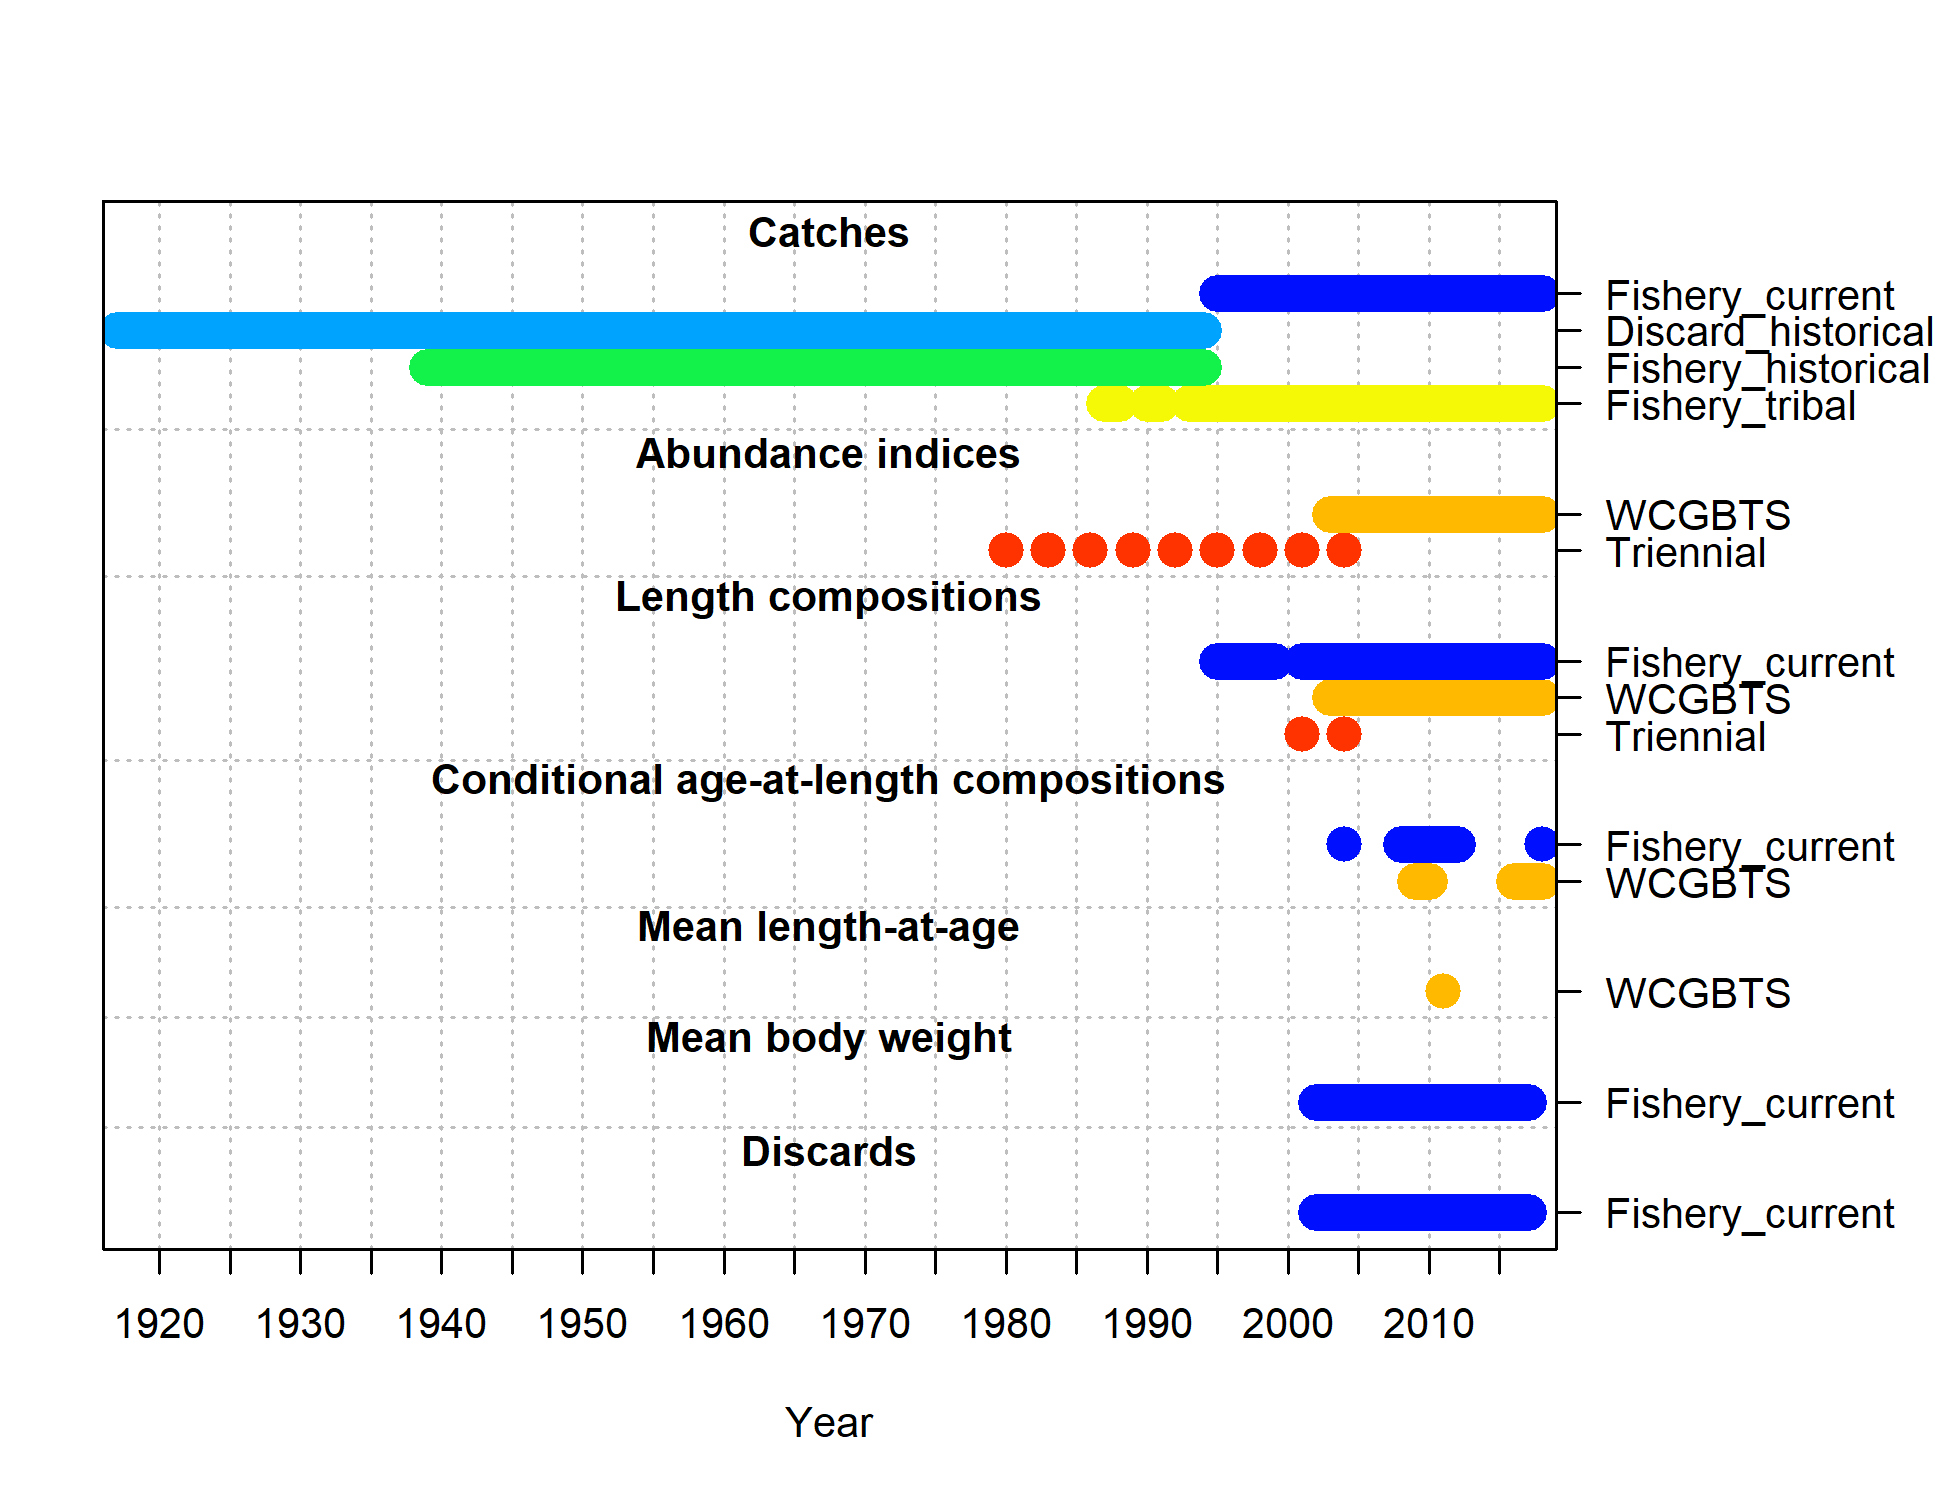
\includegraphics{r4ss/plots_mod1/data_plot.png}
\caption{Summary of data sources used in the model.}\label{fig:data_plot}
\end{centering}
\end{figure}

\newpage

\FloatBarrier

\newpage

\begin{figure}[!h]
\begin{centering}
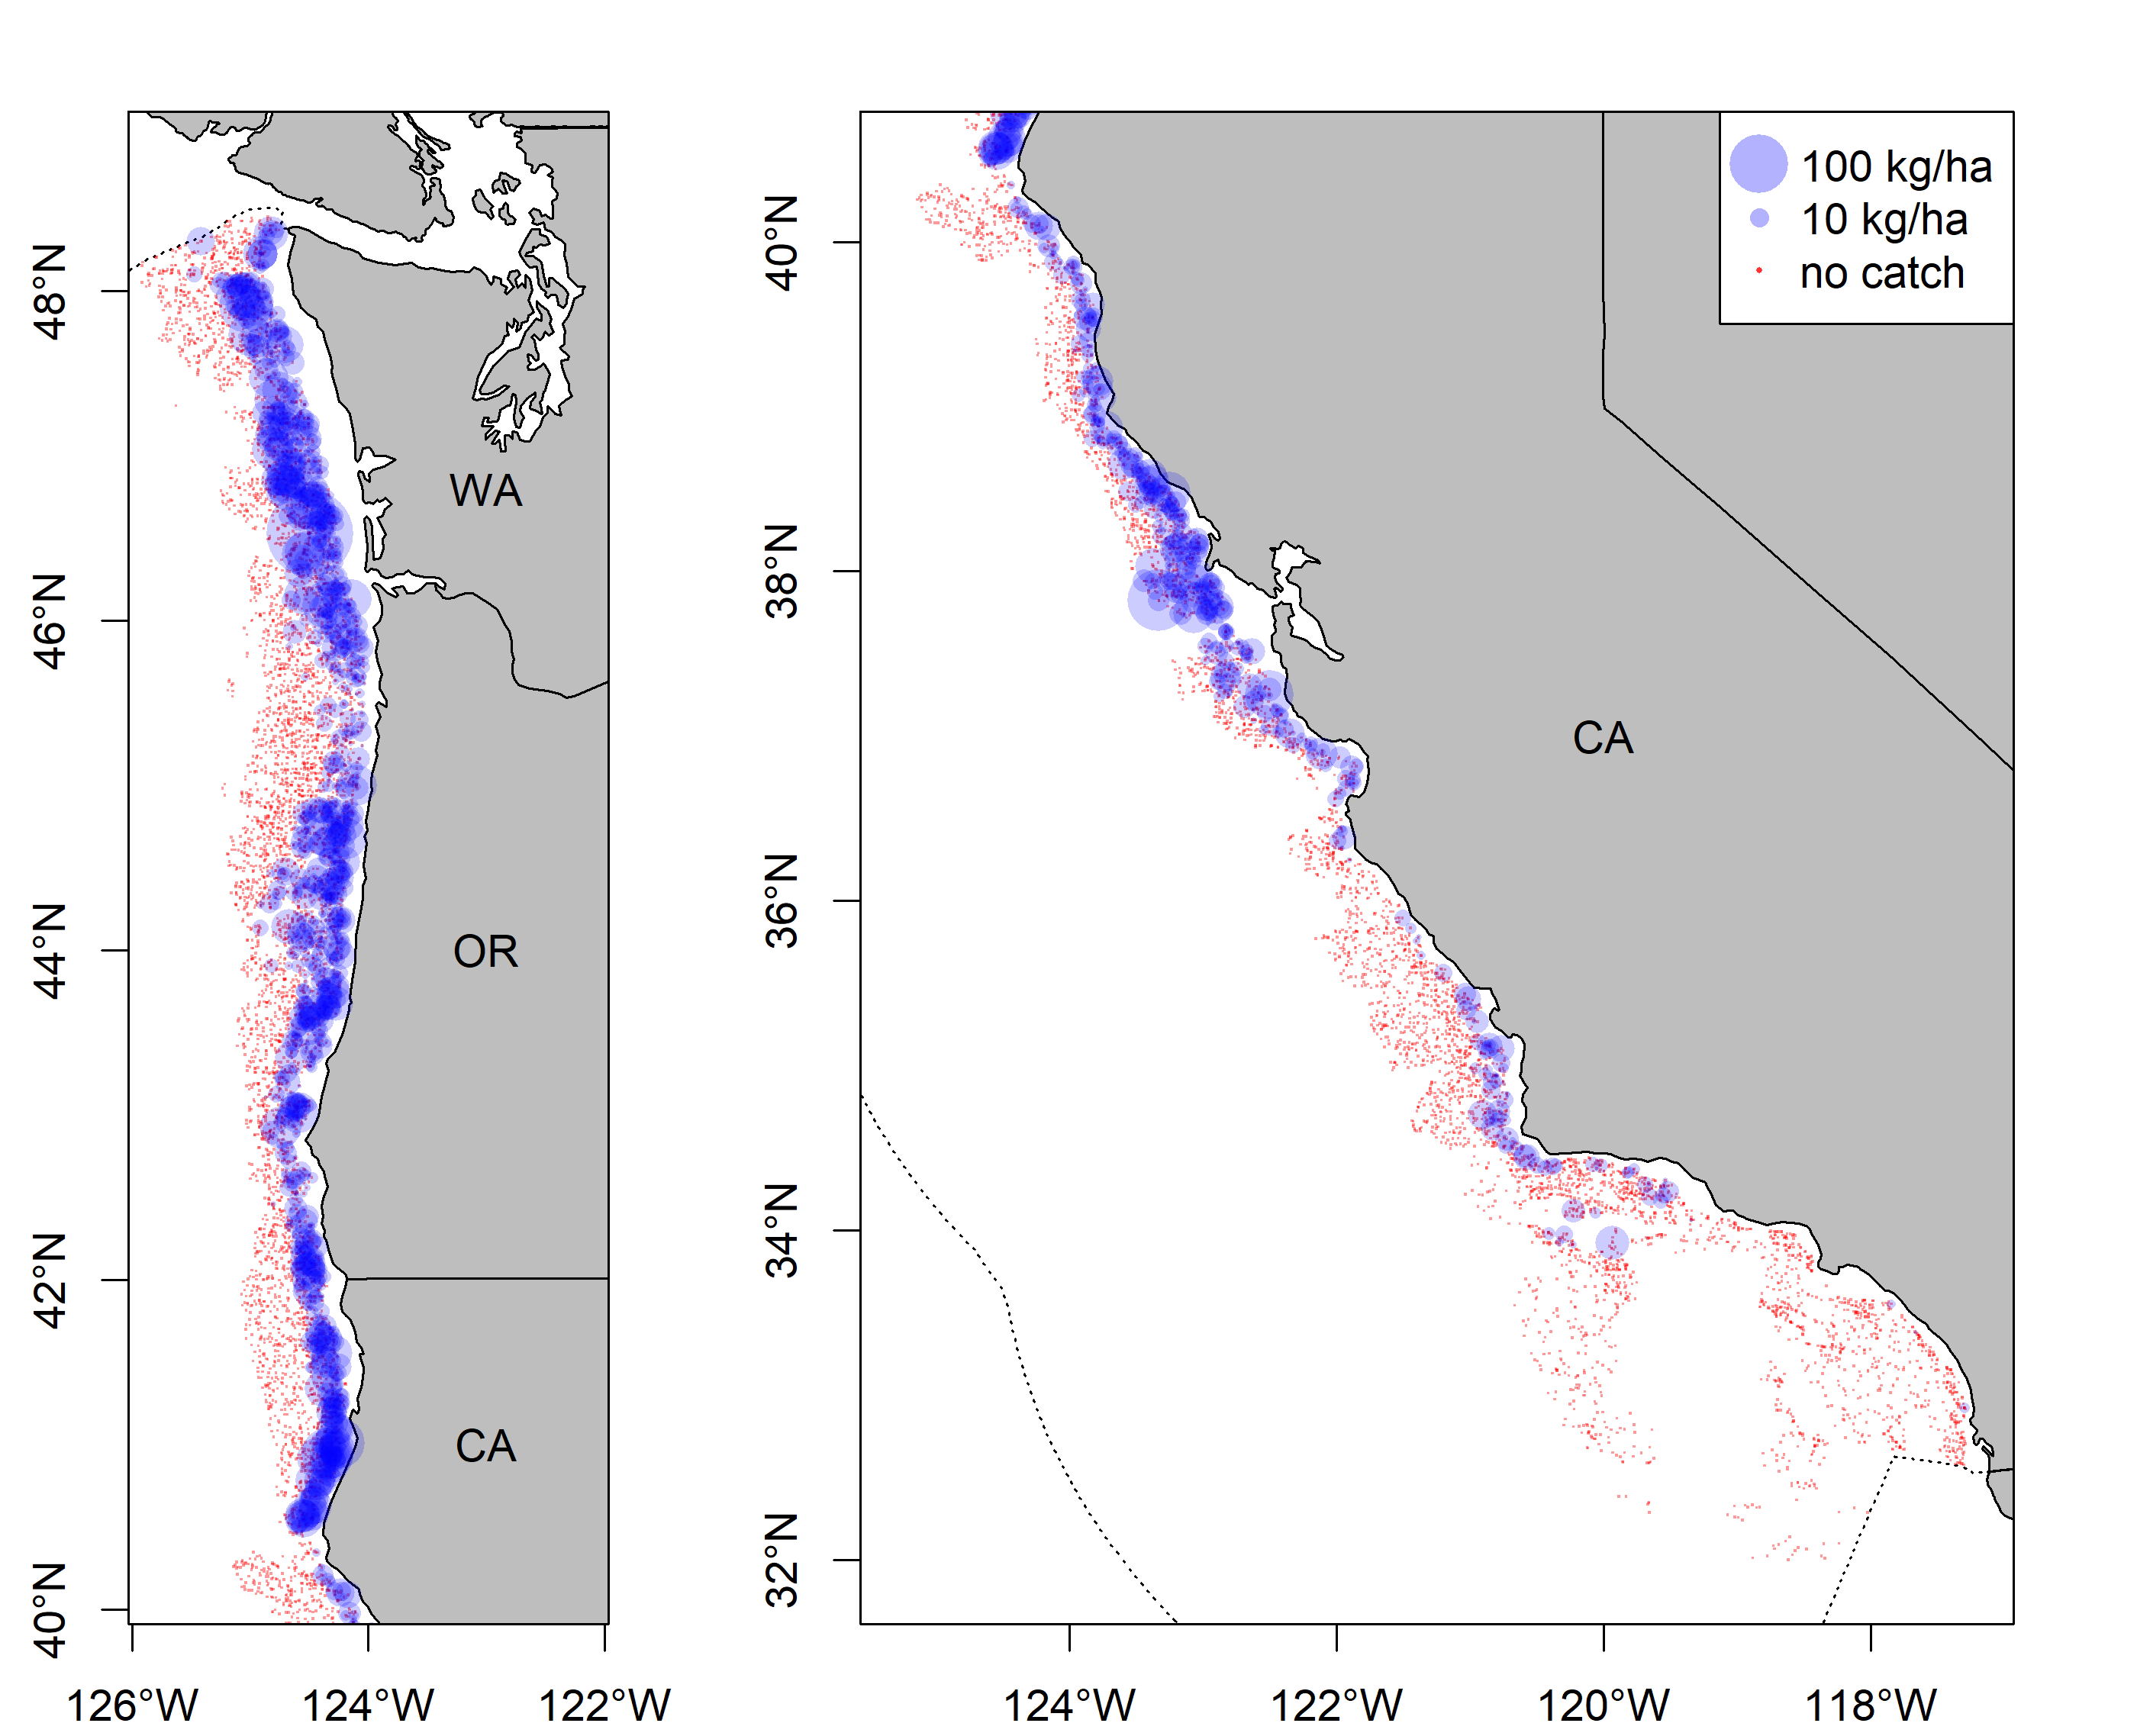
\includegraphics{Figures/survey_hauls_map.png}
\caption{Map showing the distribution of Big Skate within the area covered by the West Coast Groundfish Bottom Trawl Survey aggregated over the years 2003--2018.}\label{fig:survey_hauls_map}
\end{centering}
\end{figure}

\newpage

\FloatBarrier

\begin{figure}
\centering
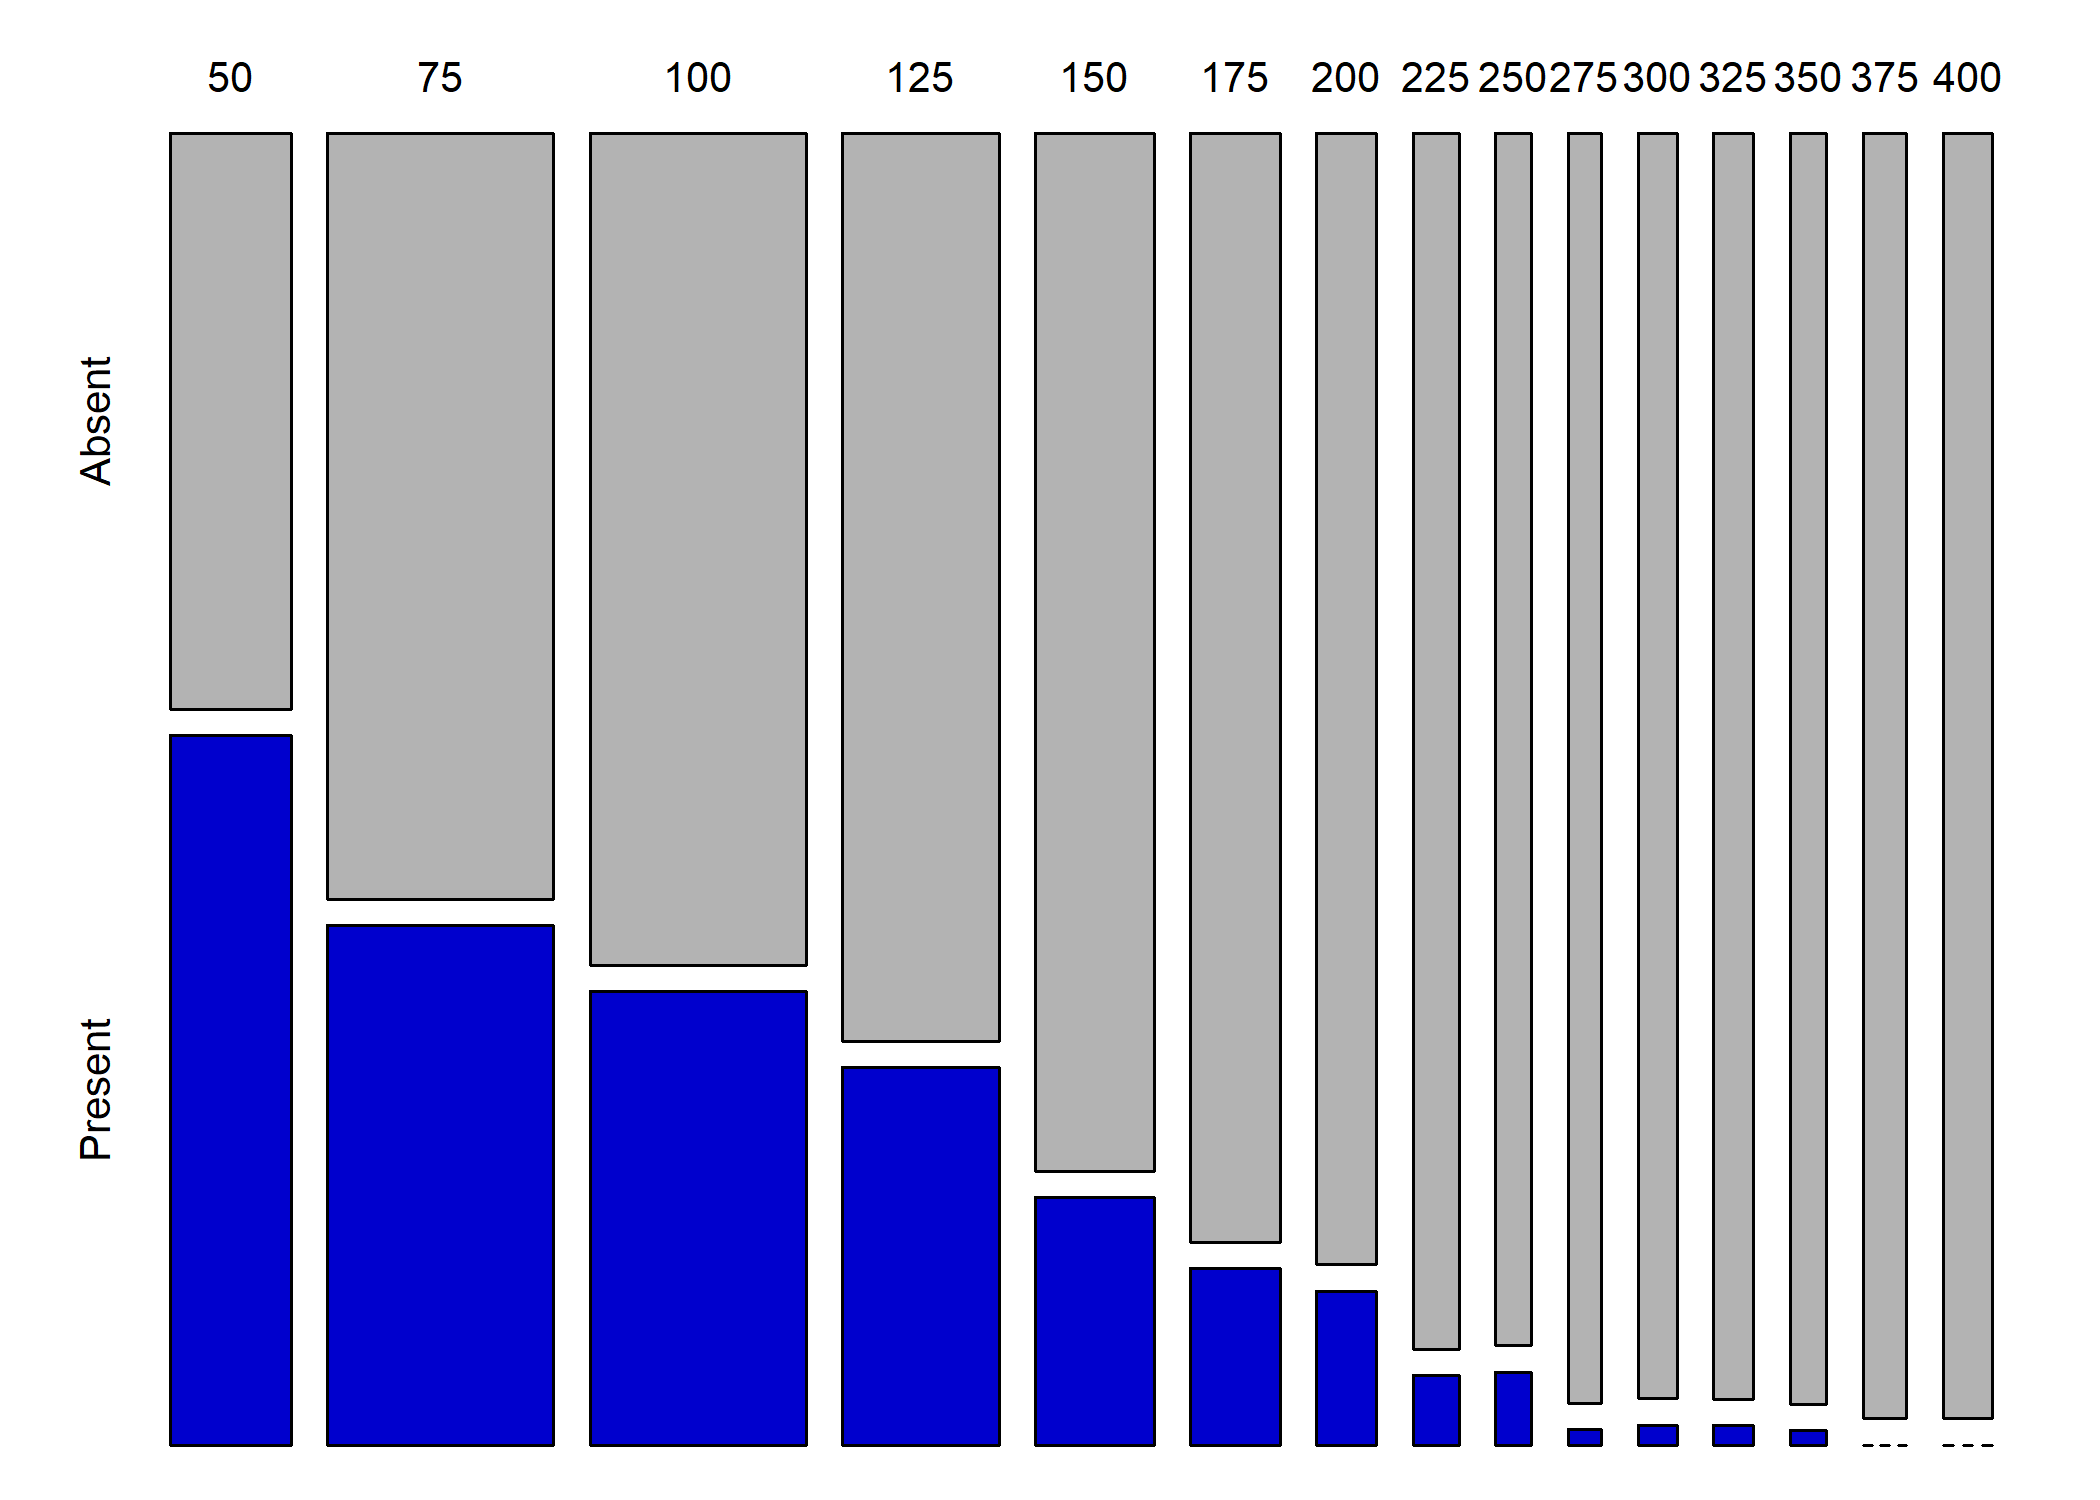
\includegraphics{Figures/WCGBTS_presence_absence_by_depth_bin.png}
\caption{Presence or absence of Big Skate in the WCGBT Survey by 25 m
depth bin for all 6,382 hauls with depth less than 425 m over the years
2003--2018. The height and width of each block are prortional to the
number of hauls within that bin. For 50--75 m, there were 324 hauls with
Big Skate present and 263 with no Big
Skate.\label{fig:WCGBTS_presence_absence_by_depth_bin}}
\end{figure}

\begin{figure}
\centering
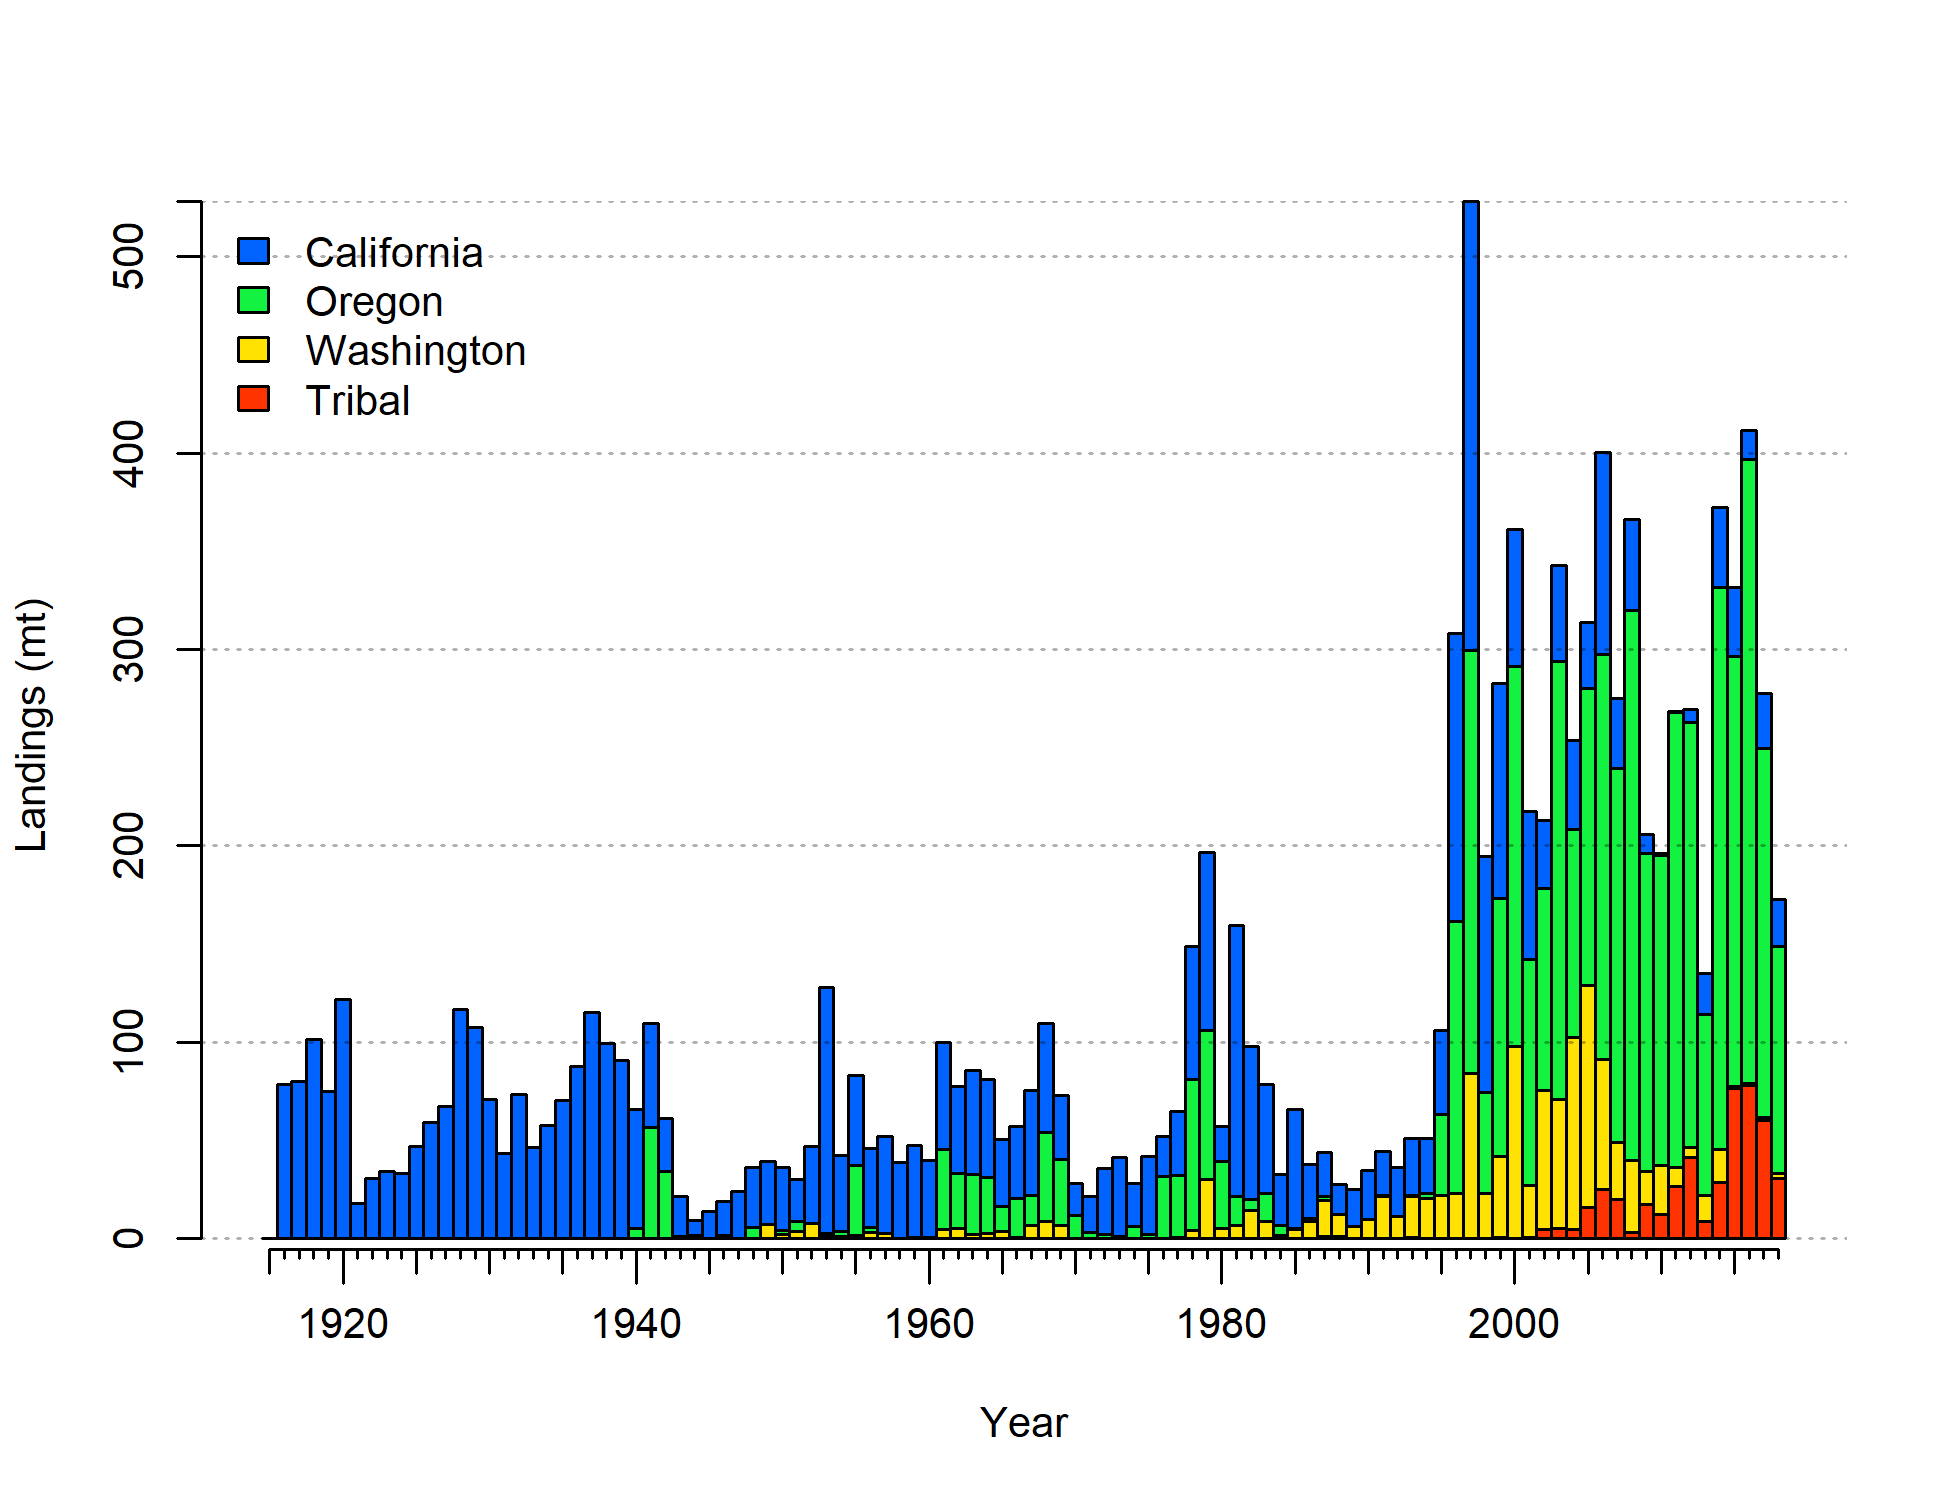
\includegraphics{Figures/catch_by_source.png}
\caption{Reconstructed landings by area. Tribal catch was all landed in
Washington. \label{fig:catch_by_state}}
\end{figure}

\begin{figure}
\centering
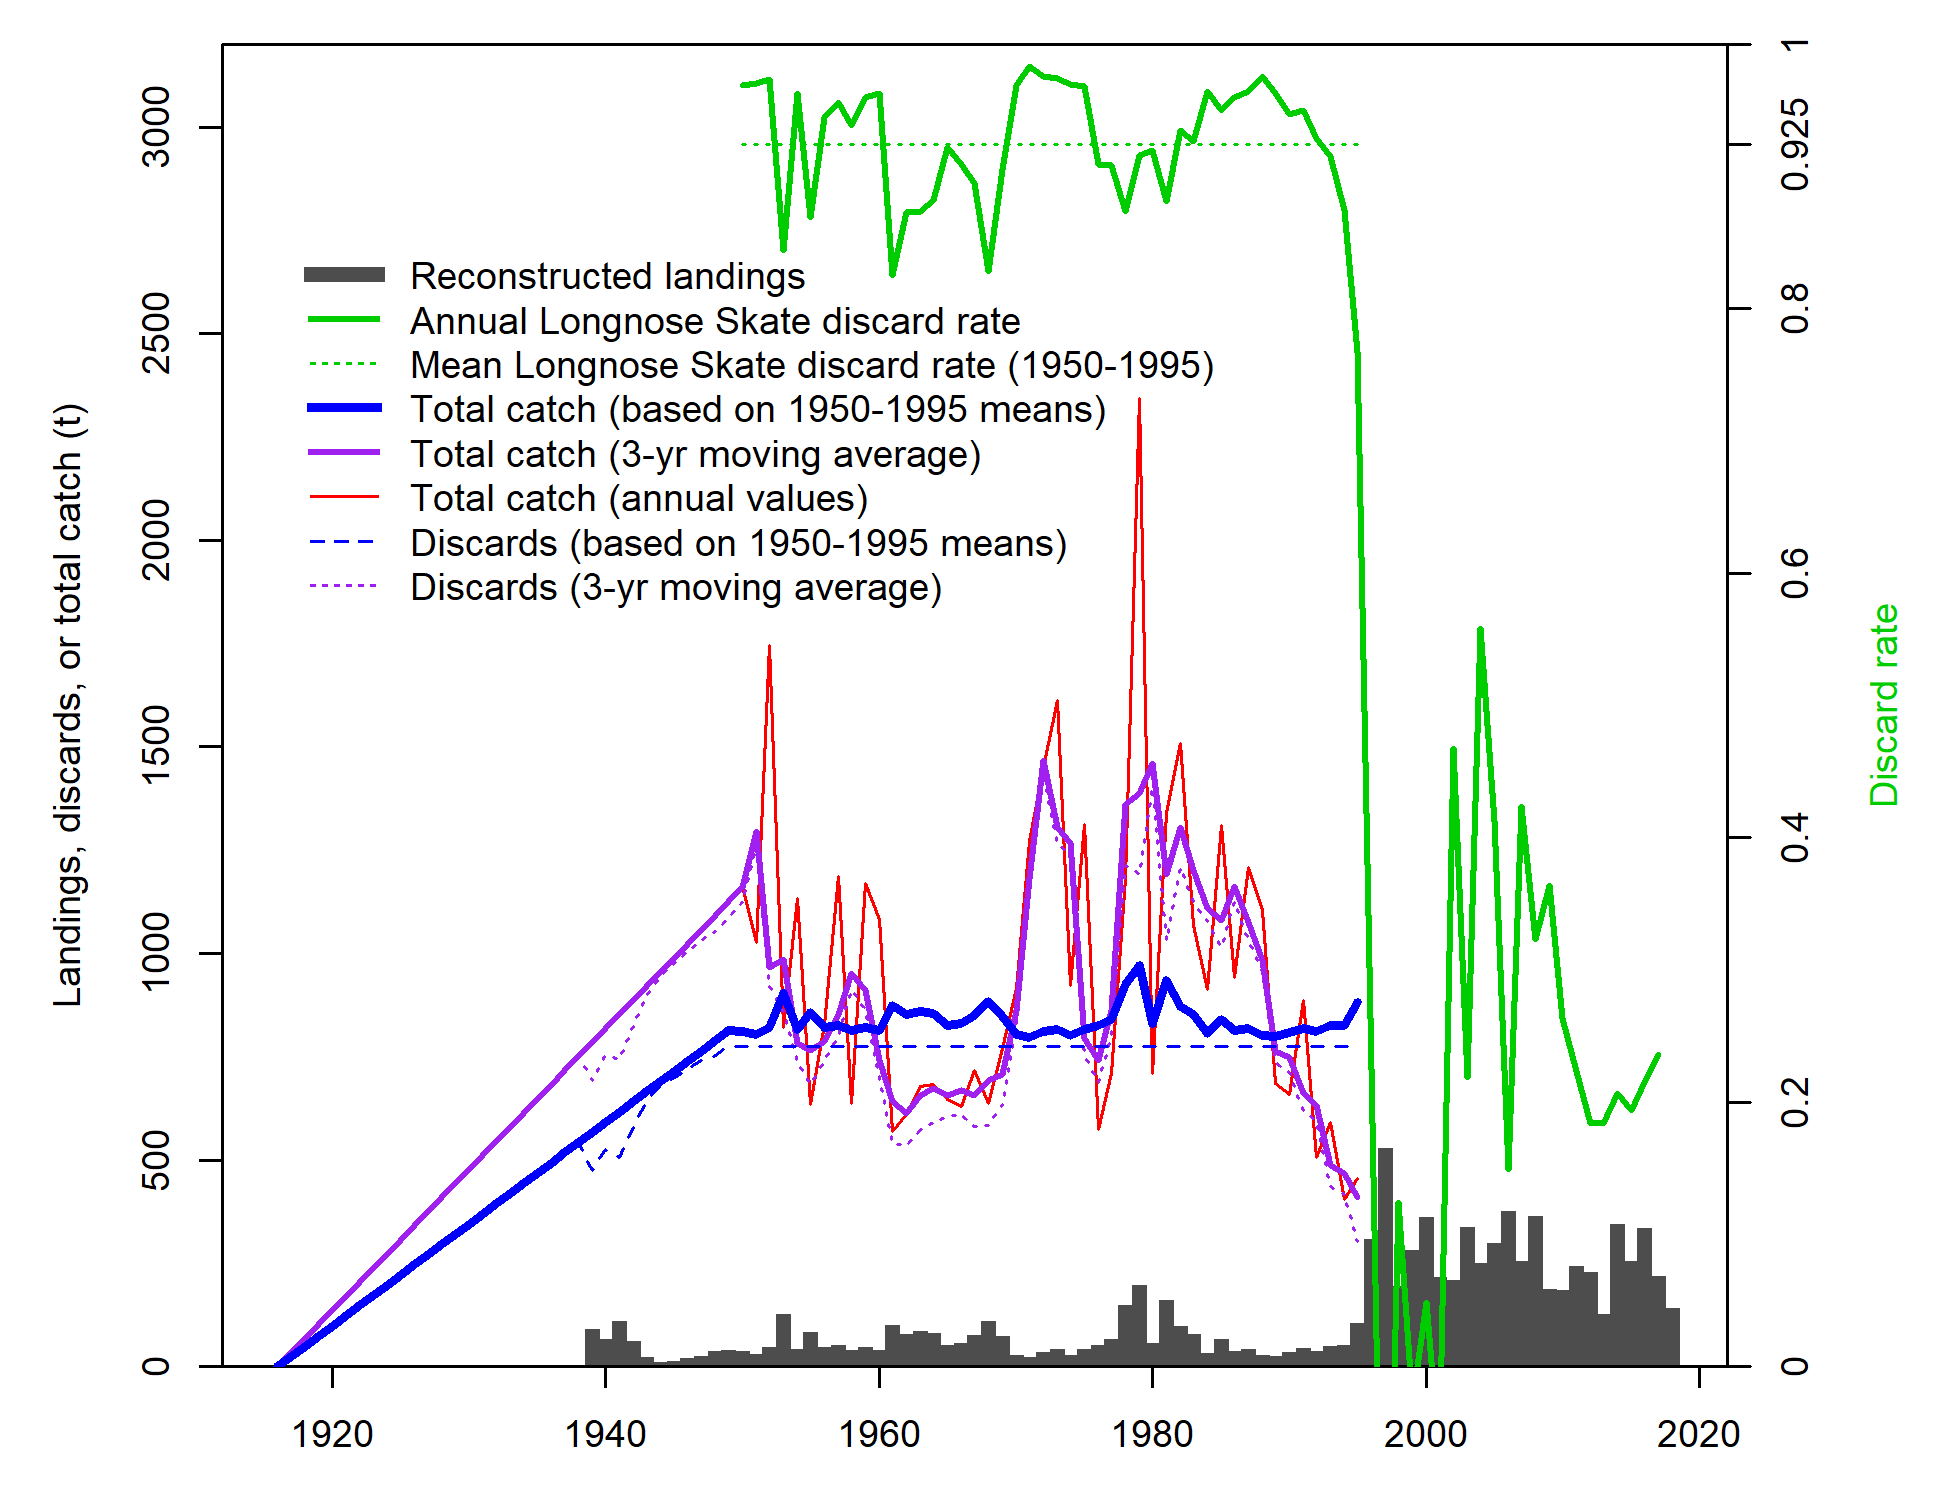
\includegraphics{Figures/discard_calculations.png}
\caption{Estimated total catch using different assumptions for discards.
The discard rates shown in green lines are relative to the right-hand
axis while all other values are relative to the left-hand
axis.\label{fig:discard_calculations}}
\end{figure}

\begin{figure}
\centering
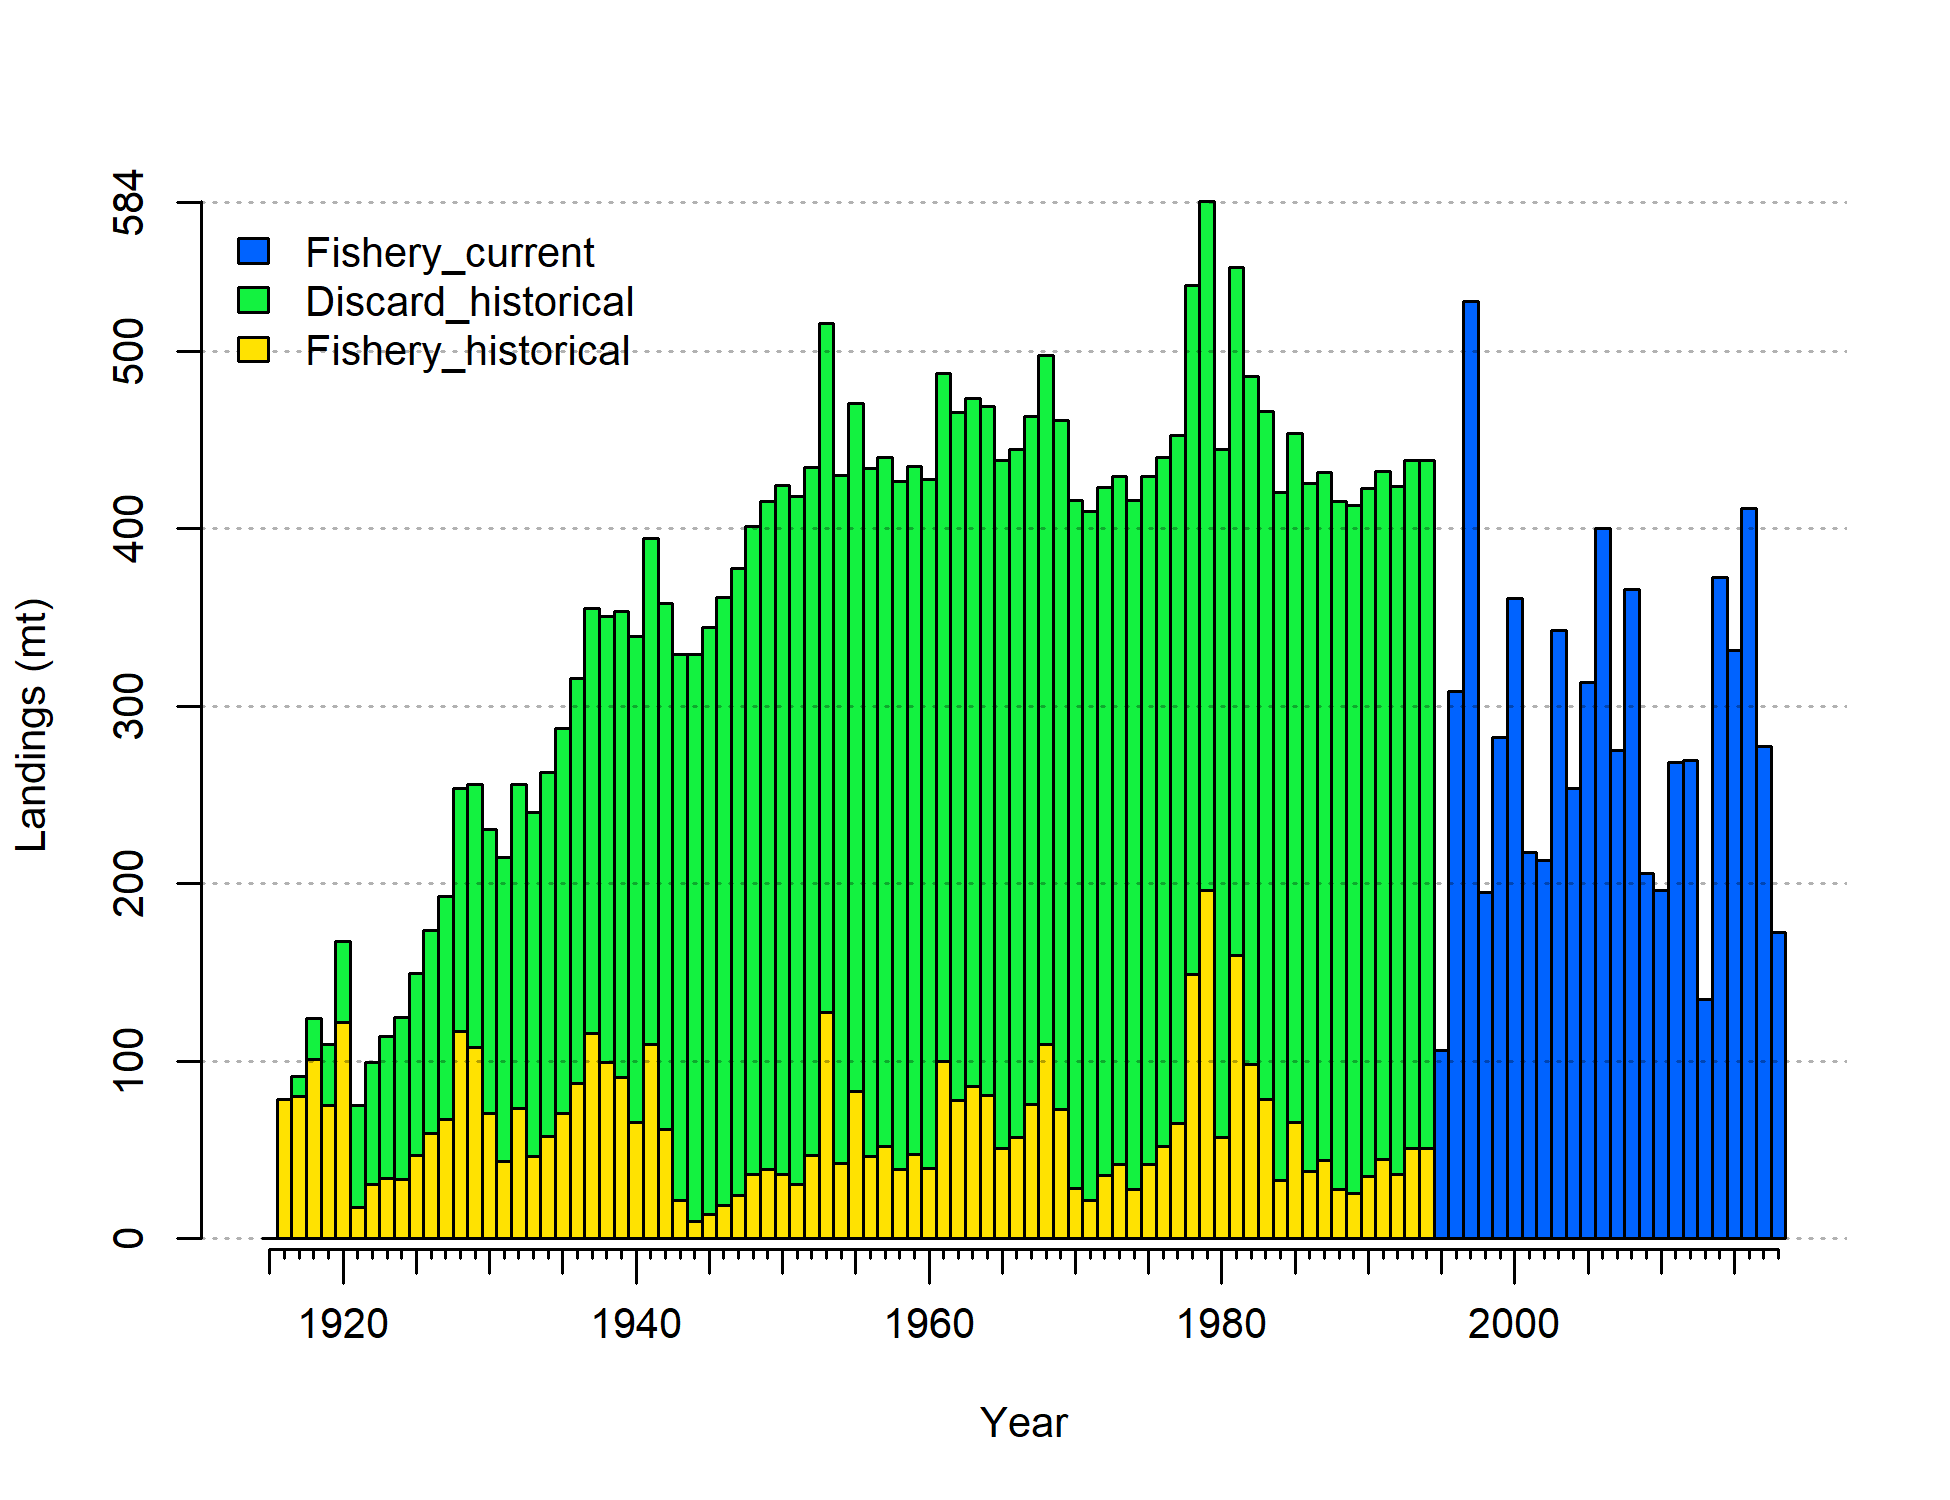
\includegraphics{r4ss/plots_mod1/catch2 landings stacked.png}
\caption{Catch data input to the model under assumed fleet structure.
The historical discards shown in green have been scaled to account for
an assumed 50\% discard mortality. Discards during the period from 1995
onward are not represented here as they are estimated within the model.
\label{fig:catch_input_plot}}
\end{figure}

\FloatBarrier

\begin{figure}
\centering
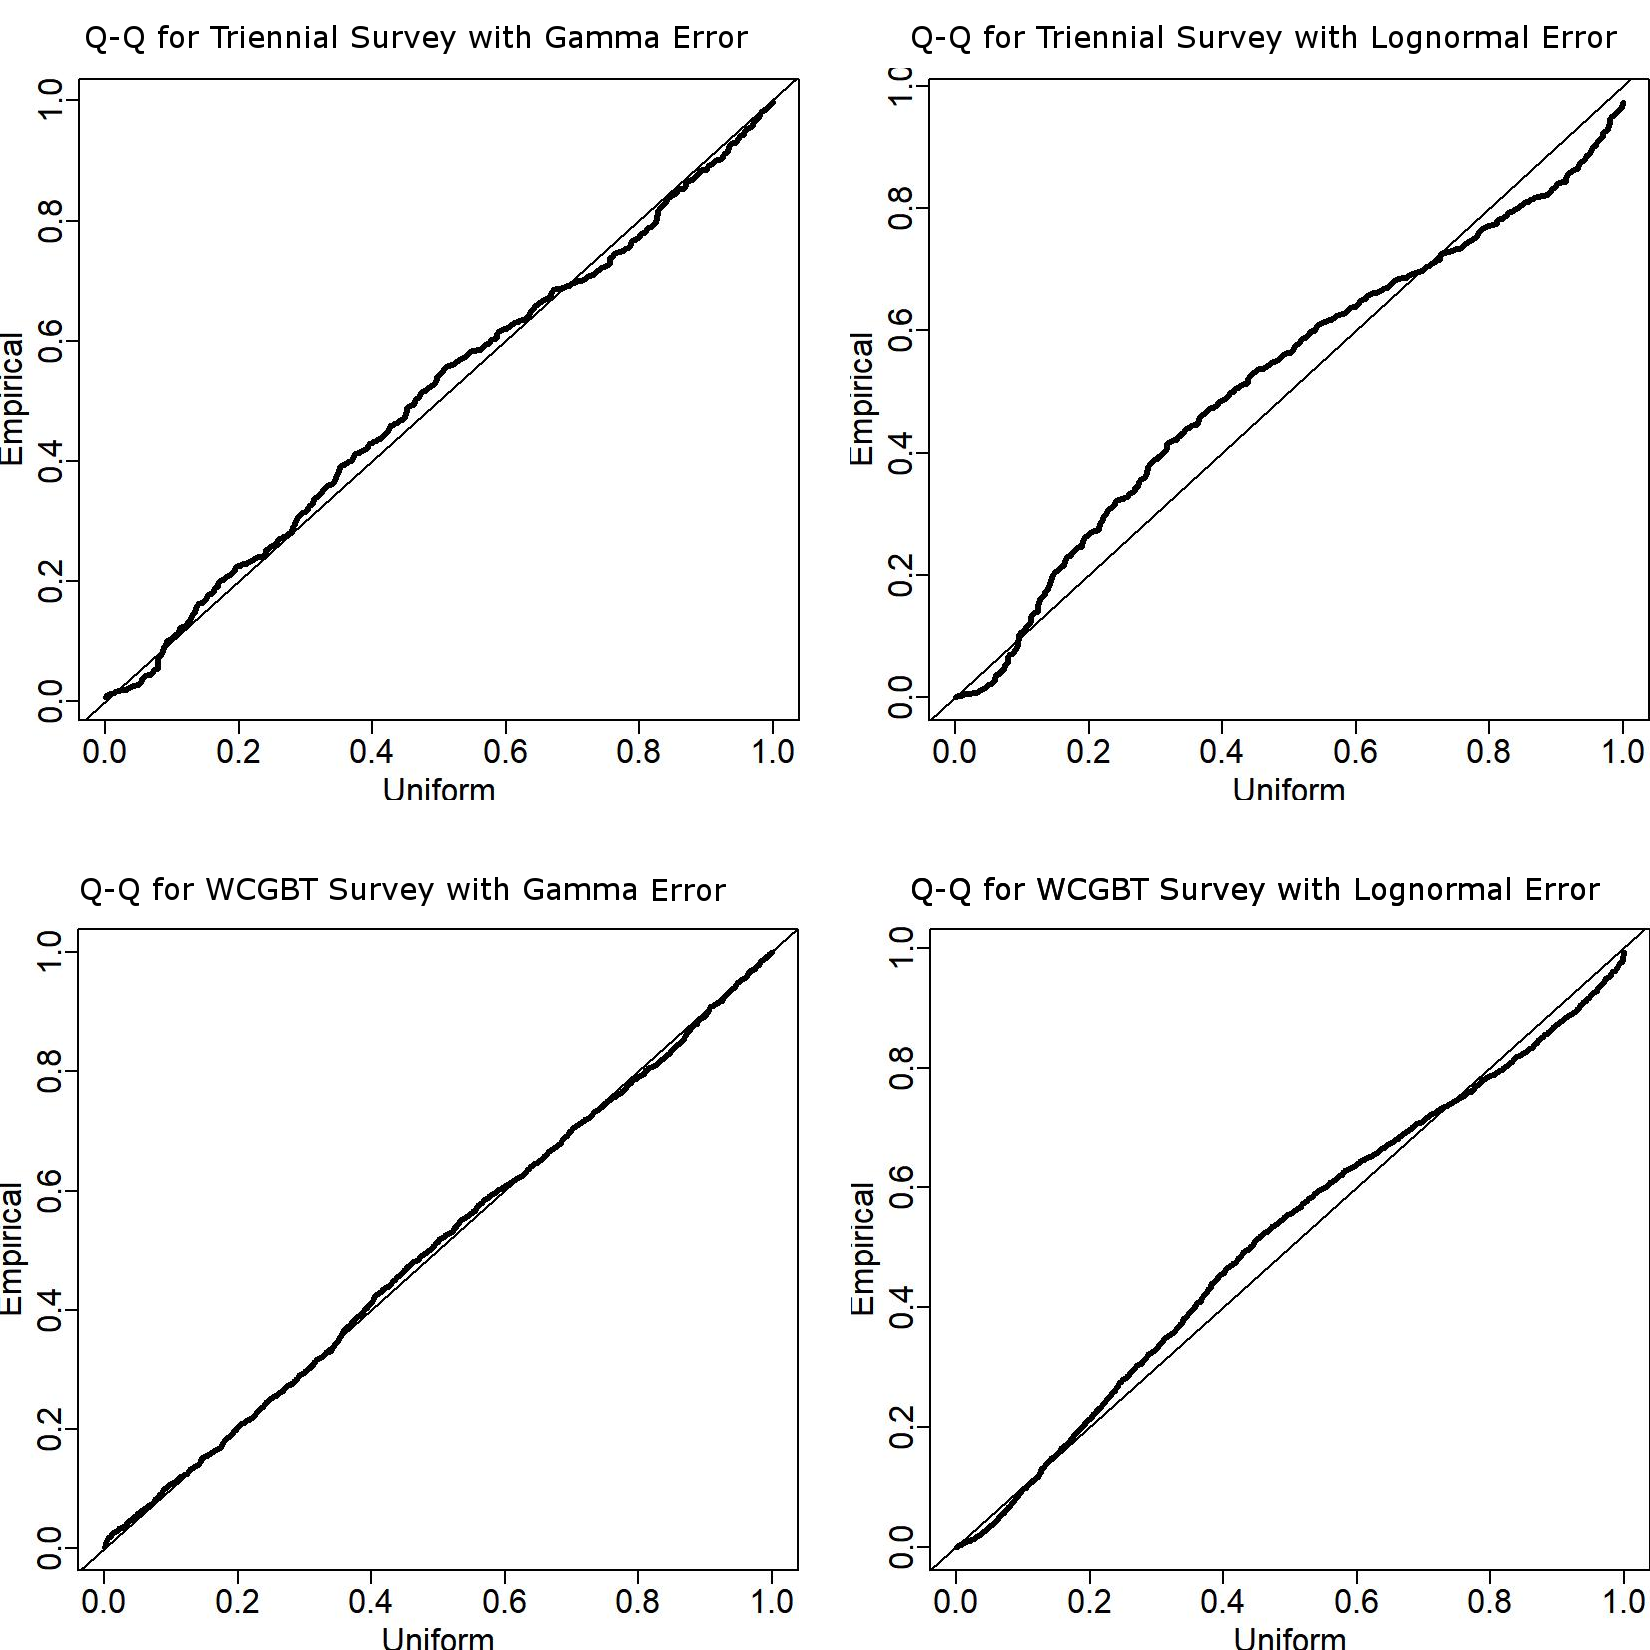
\includegraphics{Figures/VAST_QQ_plots.png}
\caption{Quantile-quantile (Q-Q) plot showing empirical quantiles of the
positive catch rate relative to their expected theoretical quantiles
within the VAST geostatistical standardization for the two surveys with
both Gamma and Lognormal error structures.\label{fig:VAST_QQ_plots}}
\end{figure}

\begin{figure}
\centering
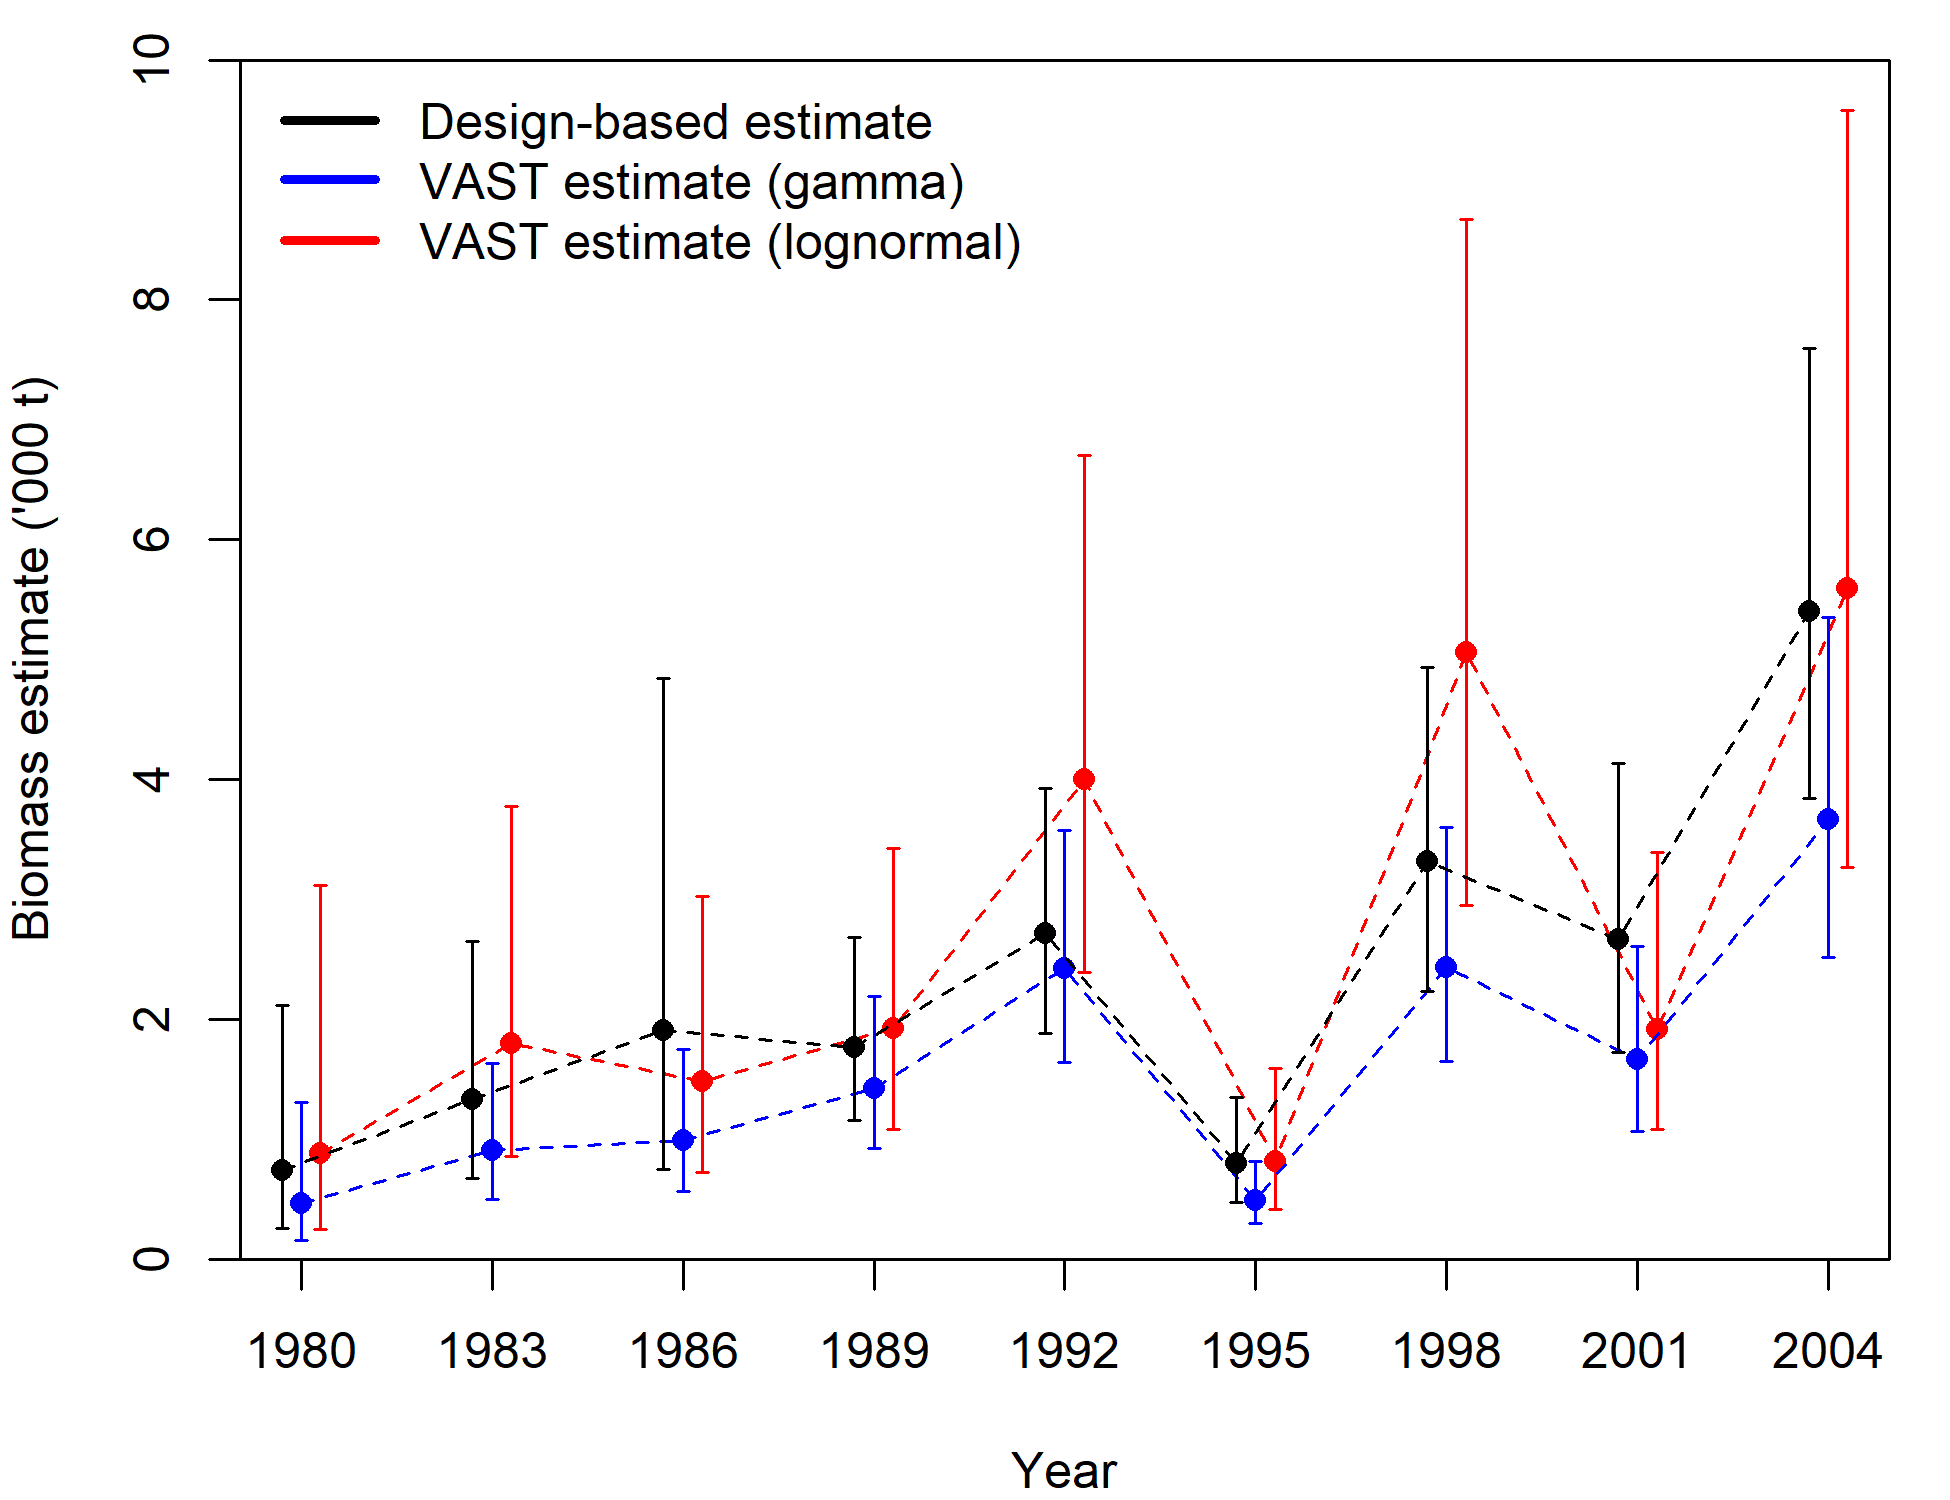
\includegraphics{Figures/Triennial_index_compare.png}
\caption{Index of abundance from the Triennial Survey calculated three
ways.\label{fig:Triennial_index_compare}}
\end{figure}

\begin{figure}
\centering
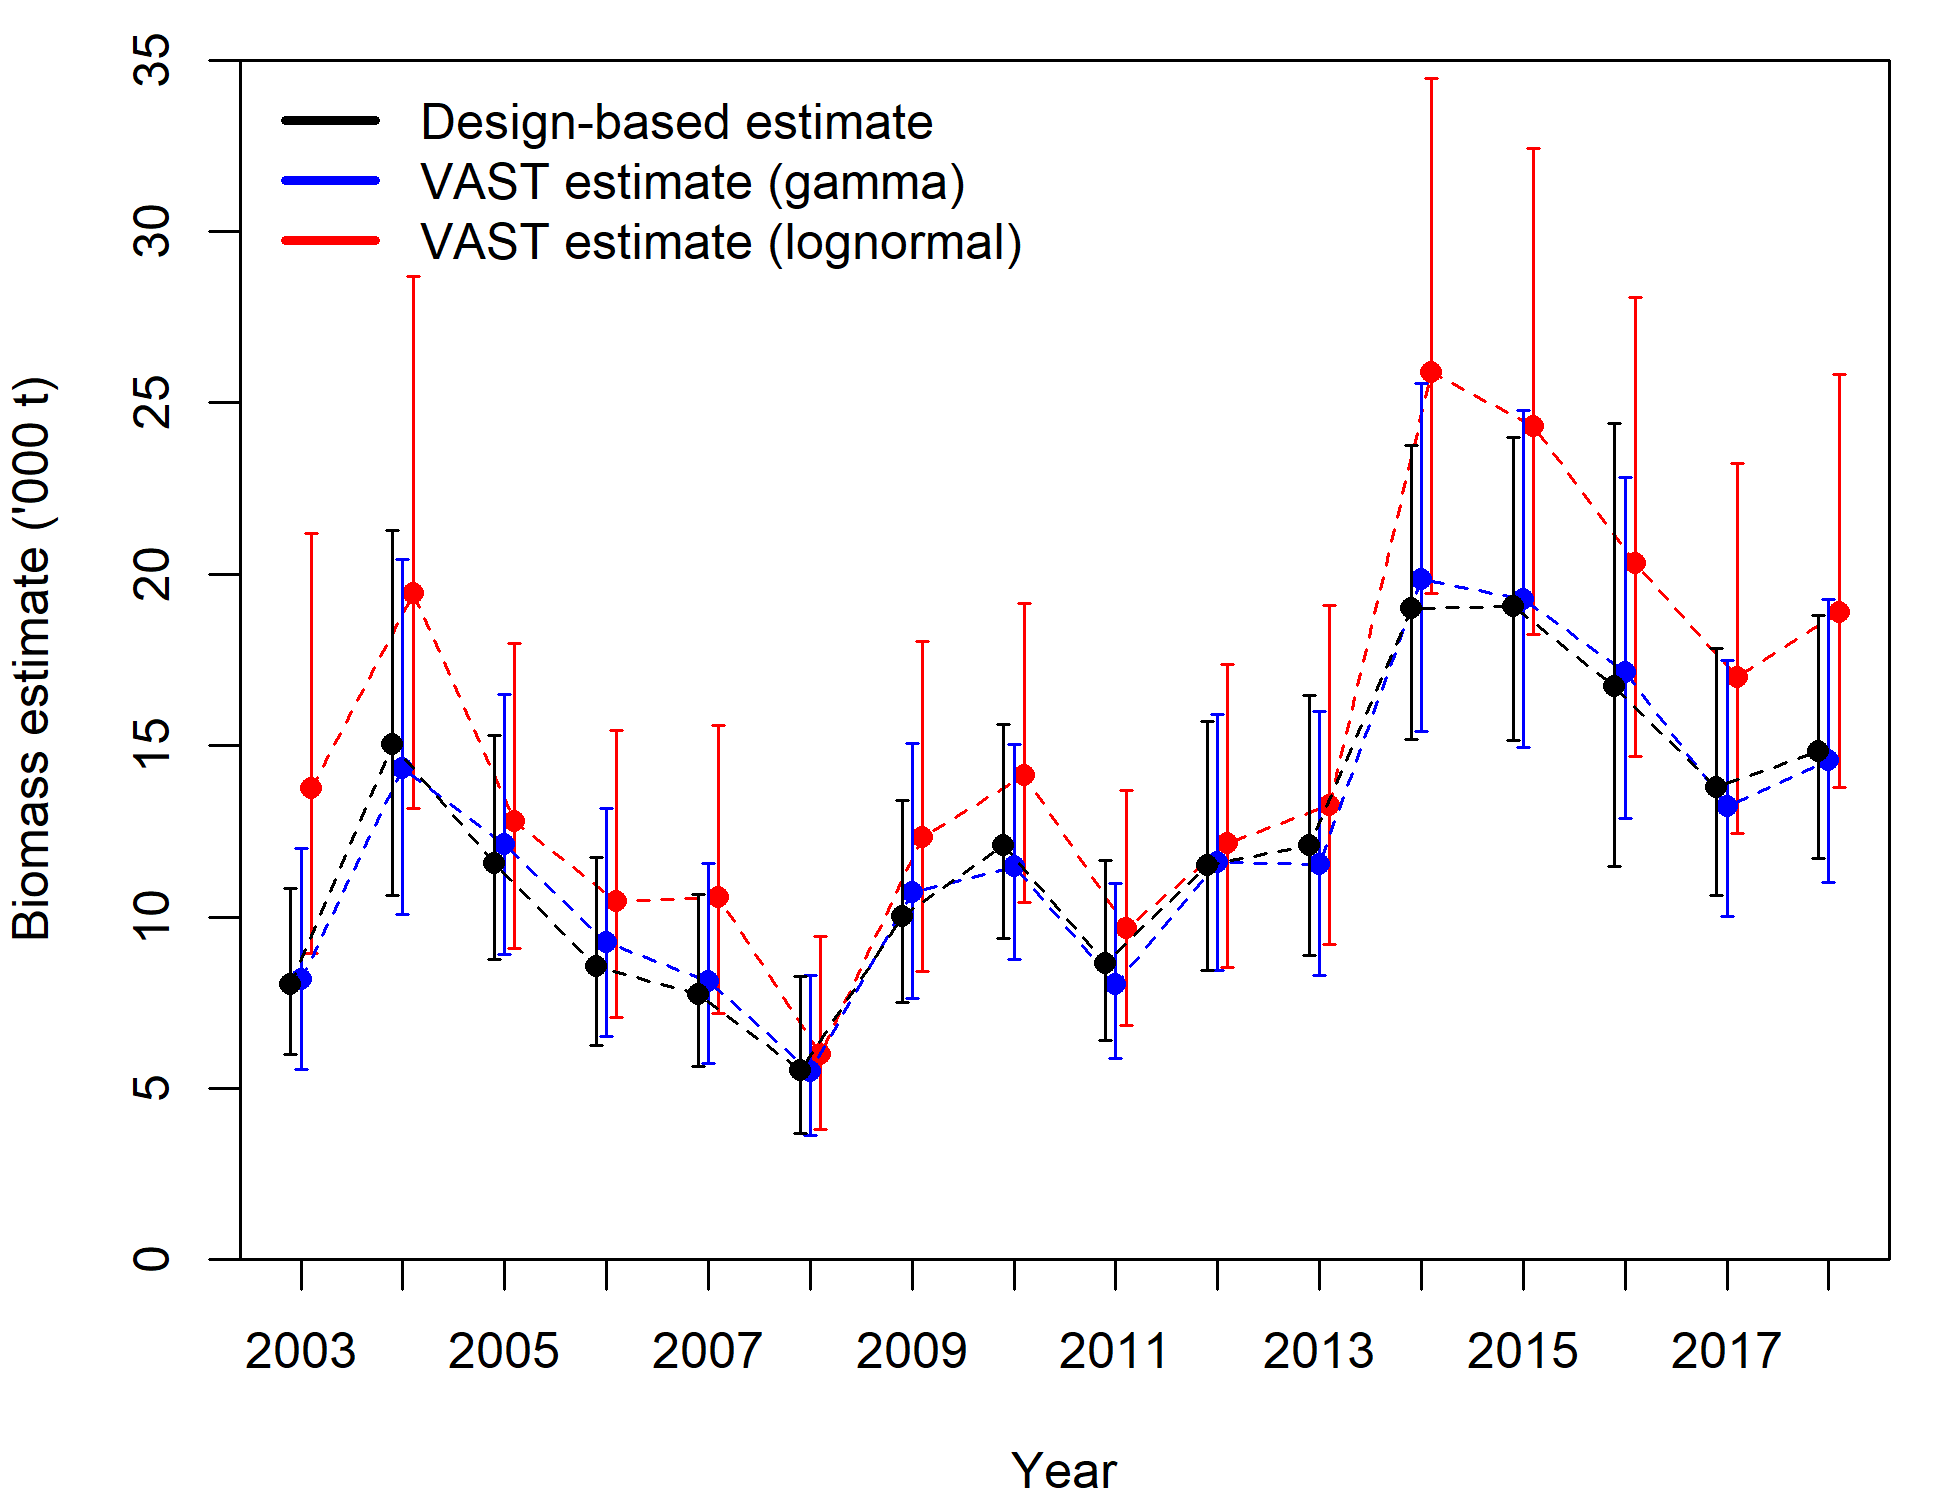
\includegraphics{Figures/WCGBTS_index_compare.png}
\caption{Index of abundance from the WCGBT Survey calculated three
ways.\label{fig:WCGBTS_index_compare}}
\end{figure}

\begin{figure}
\centering
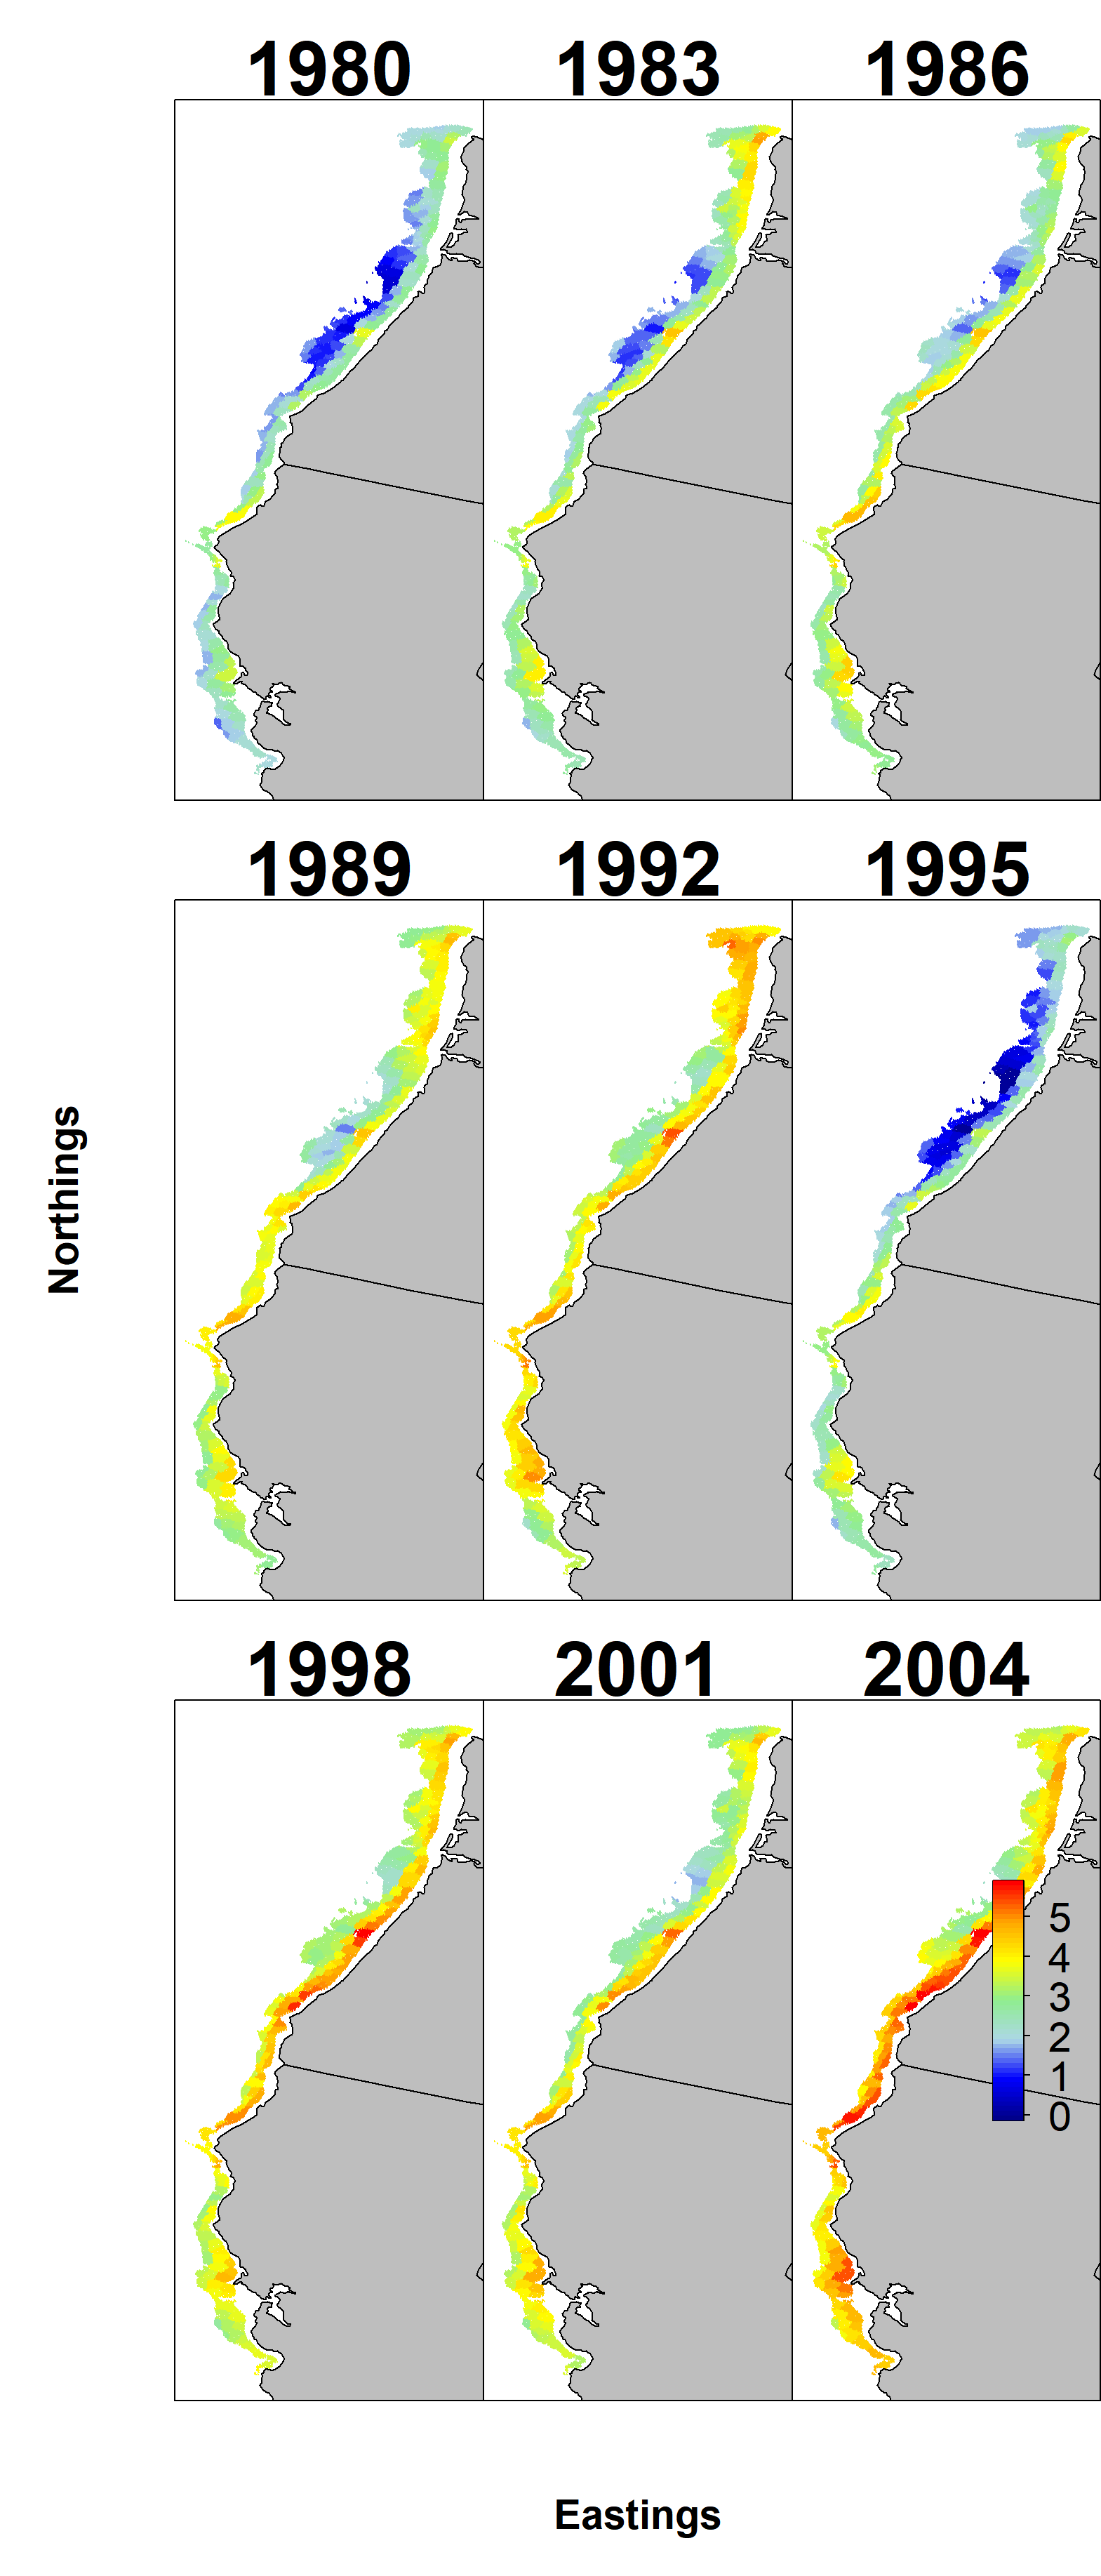
\includegraphics{Figures/VAST_Yearly_Dens_Triennial.png}
\caption{Map of estimated density by year for Big Skate in the Triennial
survey calculated using VAST with a Gamma error
structure.\label{fig:VAST_Yearly_Dens_Triennial}}
\end{figure}

\begin{figure}
\centering
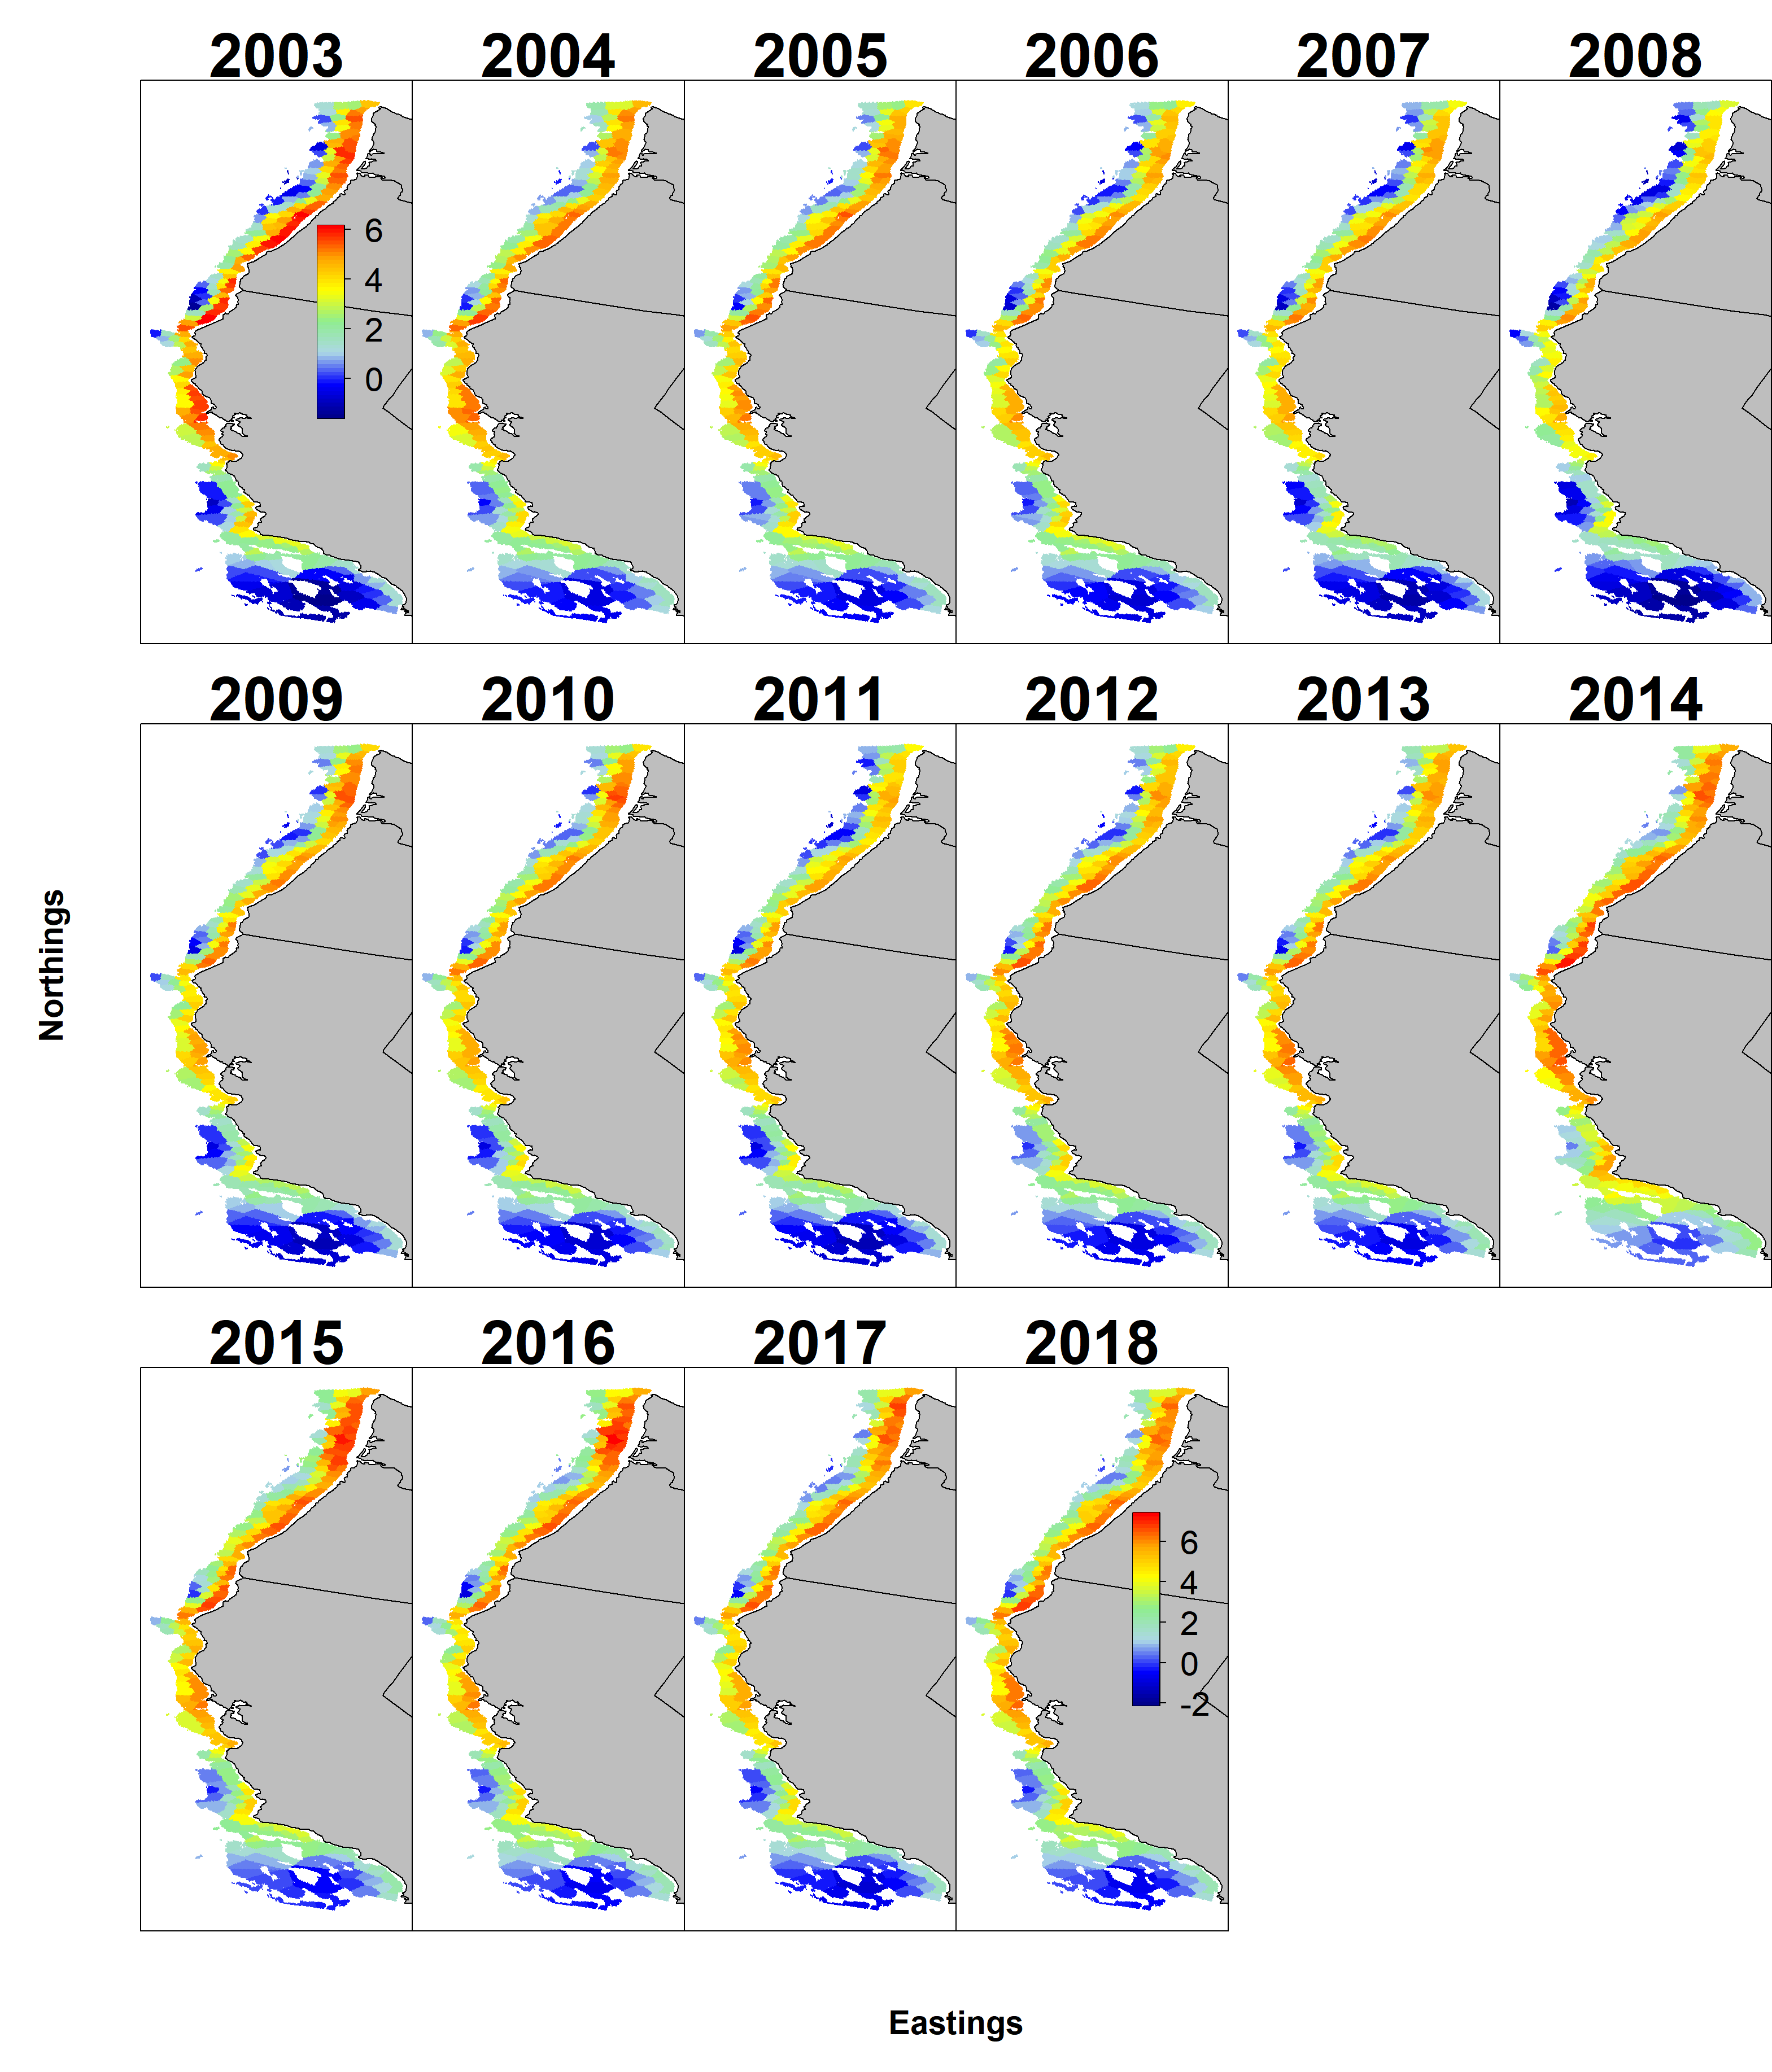
\includegraphics{Figures/VAST_Yearly_Dens_WCGBTS.png}
\caption{Map of estimated density by year for Big Skate in the WCGBT
Survey calculated using VAST with a Gamma error structure.
\label{fig:VAST_Yearly_Dens_WCGBTS}}
\end{figure}

\begin{figure}
\centering
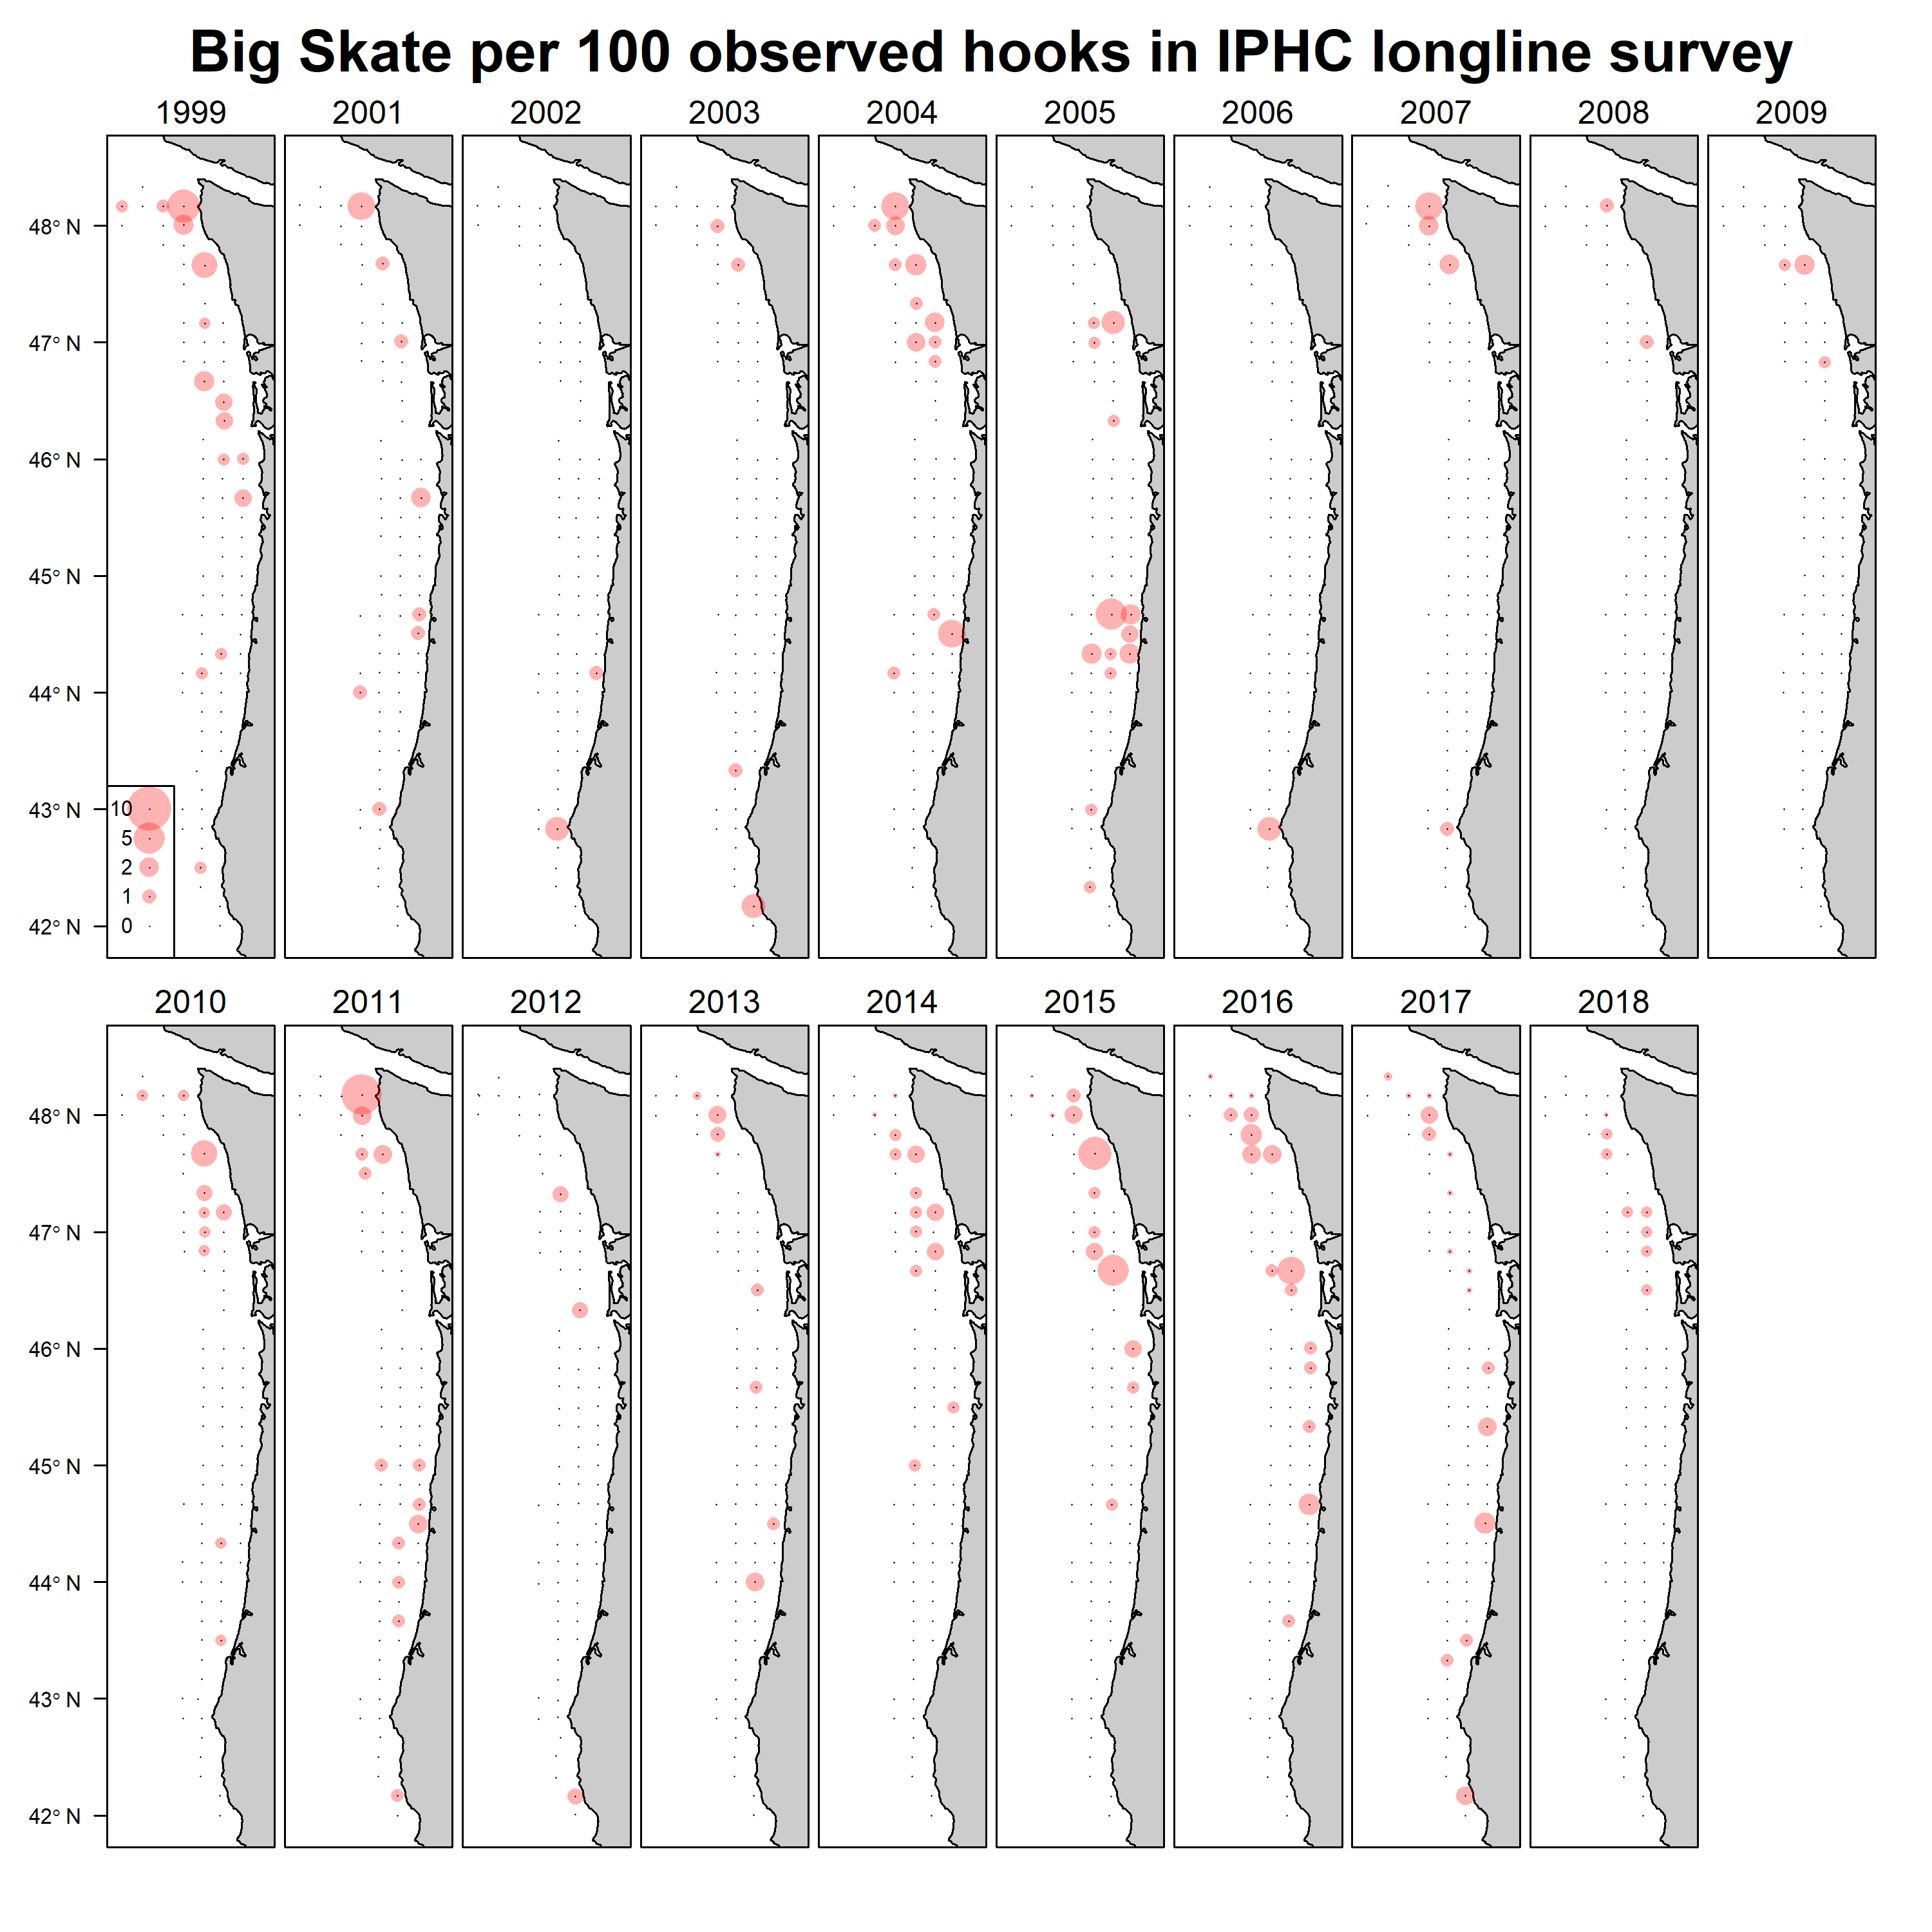
\includegraphics{Figures/IPHC_BigSkate_map.png}
\caption{Map of catch rates by year for Big Skate in the International
Pacific Halibut Commission longline survey. \label{fig:IPHC_map}}
\end{figure}

\FloatBarrier

\FloatBarrier

\FloatBarrier

\FloatBarrier

\FloatBarrier

\FloatBarrier


\end{document}
